\documentclass[11pt,a4paper]{report}

% Packages 

\usepackage[francais]{babel}
\usepackage[utf8]{inputenc}

\usepackage{amsmath}
\usepackage{amsfonts}
\usepackage{amssymb}
\usepackage{makeidx}
\usepackage{graphicx}
\usepackage{afterpage}
\usepackage{cite}
\usepackage{longtable}

\usepackage[section]{placeins}
\usepackage{float}
\usepackage{listings}
\usepackage{color}

\usepackage{booktabs} % To thicken table lines
\usepackage{pgfplotstable}
\usepackage[final]{pdfpages}


\usepackage[hidelinks]{hyperref}
\usepackage{minitoc}

\usepackage{cleveref}


\lstset{frame=tb,
	language=R,
	keywordstyle=\color{blue},
	alsoletter={.}
}

\usepackage{enumitem}
\renewcommand\descriptionlabel[1]{\textbf{#1 :}}

\usepackage{subfig}
\usepackage{graphicx}

\usepackage{array}

% Evite les gros début de chapitre inutiles. 
\usepackage{titlesec}

% niveaux de table des matières
\setcounter{secnumdepth}{4}
\setcounter{tocdepth}{3}

% Liste des abréviations
\usepackage{nomencl} 
\makenomenclature 
\renewcommand{\nomname}{Liste des abréviations}% Pour redéfinir le titre De cette liste





\makeatletter

\newif\if@mainmatter \@mainmattertrue

\newcommand\frontmatter{%
	\cleardoublepage
	\@mainmatterfalse
	\pagenumbering{roman}}
\newcommand\mainmatter{%
	\cleardoublepage
	\@mainmattertrue
	\pagenumbering{arabic}}
\newcommand\backmatter{%
	\if@openright
	\cleardoublepage
	\else
	\clearpage
	\fi
	% \@mainmatterfalse
}
\makeatother


\titleformat{\chapter}
{\normalfont\LARGE\bfseries}{\thechapter}{1em}{}
\titlespacing*{\chapter}{0pt}{3.5ex plus 1ex minus .2ex}{2.3ex plus .2ex}

% Modification de commandes 

\newcommand\blankpage{%
	\null
	\thispagestyle{empty}%
	\addtocounter{page}{-1}%
	\newpage}

\graphicspath{ {img/} }


\author{Thibault Schowing}

%TODO Trouver un bon titre au travail
\title{Amélioration de la productivité de cultures tropicales par des méthodes d'apprentissage automatique}





\begin{document}
	% Ordre de préférence:
	% a) La page de couverture
	% b) Le cahier des charges
	% c) La table des matières
	% d) Le résumé
	% e) L'introduction
	% f) Le corps du rapport
	% g) La conclusion
	% h) La bibliographie
	% -i) La liste des symboles et abréviations utilisés
	% -j) La liste des figures
	% -k) Les annexes
	% -l) Le journal de travail
	
	% Page de titre
	
	\dominitoc

	\begin{titlepage}
		\centering
		
		\small{Haute Ecole d'Ingénierie et de Gestion du Canton de Vaud  \par}
		\footnotesize{University of Applied Sciences Western Switzerland\par}
		\vspace{1cm}
		
		
\includegraphics[width=0.5\textwidth]{HEIG-VDLogo}\par
		
		\vspace{1cm}
		\Large{Amélioration de la productivité de cultures tropicales par des méthodes d'apprentissage automatique\par}
		\vspace{1.5cm}
		\small{Caractériser et prédire la qualité des cafés colombiens \par}
		\vspace{2cm}
		\small\textit{Thibault \textsc{Schowing}}\par
		\small{Travail de Bachelor}\par
		\small{\today\par}
		
		\vfill
		Professeur responsable: ~Carlos Andrès \textsc{Peña}\par
		Superviseur (CIAT): Sylvain \textsc{Delerce} \par
		Superviseur (CIAT): Daniel \textsc{Jimenez}
		
		
	\end{titlepage}
	
	\afterpage{\blankpage}
	\pagenumbering{gobble}
	
	\frontmatter
	
	% Entrées pour la liste des abréviations, compiler -> exécuter la commande ci-dessous -> recompiler
	
	% makeindex -s nomencl.ist -t "Bachelor_Schowing2017.nlg" -o "Bachelor_Schowing2017.nls" "Bachelor_Schowing2017.nlo"
	\nomenclature{SOM}{Self Organizing Map}
	\nomenclature{FNC}{Fédération Nationale des Caféiculteurs}
	\nomenclature{DTR}{Diurnal Temperature Range}
	\nomenclature{SICA}{Sistema de Información Cafetera}
	\nomenclature{SCAA}{Specialty Coffee Association of America}
	\nomenclature{CIAT}{Centre Internationnal de recherche pour l'Agriculture Tropicale}
	\nomenclature{tmax}{Température maximale}
	\nomenclature{tmin}{Température minimale}
	\nomenclature{tmean}{Température moyenne}
	\nomenclature{GIS}{Geographical Information System}
	\nomenclature{}{}
	
	\renewcommand{\abstractname}{Remerciements}
\begin{abstract}
	\thispagestyle{plain}
	\noindent Je tiens à adresser mes remerciements à tous ceux qui m'ont accompagné dans la réalisation de ce projet, sans eux, rien n'aurait été possible. \\
	
	\noindent Un grand merci au professeur Carlos Andrés Peña, qui m'a donné l'opportunité de sortir des sentiers battus et de découvrir un environnement de travail exceptionnel à Cali en Colombie. C'est une expérience que je ne suis pas près d'oublier et qui va sans doute longtemps me suivre dans mon parcours professionnel et personnel.\\
	
	\noindent Merci à Sylvain, Hugo et Daniel qui m'ont guidé à travers ce projet grâce à leur grande expérience dans le domaine. Grâce à vous j'ai appris énormément et ce bagage me sera d'une grande utilité dans le futur.\\

	\noindent Merci à la famille et aux amis pour leur temps de relecture et leur patience.\\
	
	\noindent Et enfin, un grand merci à Fanny, Alexandra, Hugo, Andrés, Steven et tous les autres qui m'ont immédiatement accepté et avec qui j'ai vécu une grande aventure de deux mois, du Pacifique aux montagnes de l'axe du café. 
	
	% Une petite citation ça serait cool, mais à part "garbage in garbage out" je vois pas.
	
\end{abstract}
	\afterpage{\blankpage}
	
	\renewcommand{\abstractname}{Cahier des Charges}
\begin{abstract}
	
	\paragraph*{Objectifs} Dans un premier temps, l'objectif est de catégoriser les différents cafés en tentant de trouver des tendances gustatives par rapport aux conditions de culture. Dans un second temps, il faudra pouvoir prédire la qualité en bouche des cafés par rapport aux conditions environnementales. 
	
	\paragraph*{Tâches}
	\begin{itemize}
		\item Analyse du problème et planification des étapes du projet
		\item Analyse du contexte technique et scientifique ainsi que de l'état de l'art
		\item Décomposition du problème et conception de la solution
		\begin{enumerate}
			\item Prise en main et analyse des données disponibles
			\item Analyse et sélection des méthodes de modélisation
			\begin{enumerate}
				\item Méthodes pour la caractérisation
				\item Méthodes pour la prédiction
			\end{enumerate}
		\end{enumerate}
	\item Réalisation, implémentation et tests
	\begin{enumerate}
		\item Implémentation des méthodes pour la caractérisation (par ex. Clustering, PCA, SOM, ...)
		\item Implémentation des méthodes pour la prédiction (par ex. Réseaux de neurones, Random Forest, Logique floue,...)
	\end{enumerate}

	\item Analyse des informations obtenues et discussion des résultats
	
	\item Document et présentation
	\end{itemize}
	
\end{abstract}












	\afterpage{\blankpage}
	
	
	%\section*{Résumé}
%TODO résumé
%Résumé
\renewcommand{\abstractname}{Résumé}
\begin{abstract}
	
	
	\paragraph{Contexte} Le \textit{Centro Internacional de Agricultura Tropical } (CIAT) est un centre de recherche international qui travaille dans le but d’améliorer la productivité et la gestion de l’agriculture en zone tropicale. Ses bureaux se trouvent à Cali, en Colombie. À 200 kilomètres du centre, dans l'\textit{Eje Cafetero}, une région réputée pour la qualité de ses cafés, le comité des caféiculteurs du département de Risaralda souhaite pouvoir expliquer les différents traits de la qualité en bouche des cafés produits dans les différents secteurs de leur département. La filière café colombienne est en effet en concurrence avec d’autres pays exportateurs sur le marché international, et un des avantages comparatifs de la Colombie est que ses terroirs produisent des cafés de qualité et de caractères affirmés. Il est donc stratégique pour la fédération des caféiculteurs de Colombie d'être en mesure de faire valoir ces spécificités pour aller chercher la valeur ajoutée associée aux produits démarqués du lot.\\
	
	\paragraph{Problématique} Les membres du comité souhaitent savoir s'il est possible de caractériser les différents cafés du département par rapport aux conditions spécifiques de culture des fermes réparties sur le territoire. Les conditions de culture sont définies par des données climatiques, géographiques et des données sur la composition et la structure du sol alors que les données sur les cafés sont sous la forme de résultats de dégustations, suivant les standards de notation de la Specialty Coffee Association of America.
	
	\paragraph{Objectif}  Le but de ce travail est d'utiliser des outils de Machine Learning afin de trouver des relations entre les conditions de culture et la qualité des cafés pour découvrir d'éventuelles particularités spécifiques à certaines régions ou conditions de culture. Une fois ceci fait, l'objectif est d'explorer les possibilités de prédiction dans le but de pouvoir anticiper, comprendre et modifier les facteurs influençant sur la qualité des cafés. 
	
	
\end{abstract}



	\afterpage{\blankpage}
	
	\tableofcontents
	
	

	
	\mainmatter
	
\chapter{Introduction}
\section{Question de recherche}

%TODO enlever le "pratiques culturales", on a pas de données
A partir de données sur le climat, la qualité du sol et les pratiques culturales, est-il possible d’expliquer et de prédire les différents traits de la qualité en bouche des cafés du département de Risaralda ?


\section{Contexte du projet}
Le sujet de ce Travail de Bachelor a été proposé par le « \textit{Centro Internacional de Agricultura Tropical }» (CIAT) qui travaille dans le but d’améliorer la productivité et la gestion de l’agriculture en zone tropicale, et dont les bureaux se trouvent à Cali, en Colombie.\\

\noindent À 200 kilomètres de Cali, le comité des caféiculteurs de Risaralda souhaite pouvoir expliquer les différents traits de la qualité en bouche des cafés produits dans les différents secteurs de leur département. La filière café colombienne est en effet en concurrence avec d’autres pays exportateurs sur le marché international, et un des avantages comparatifs de la Colombie est que ses terroirs produisent des cafés de qualité et de caractères affirmés. Il est donc stratégique pour la fédération des caféiculteurs de Colombie d'être en mesure de faire valoir ces spécificités pour aller chercher la valeur ajoutée associée aux produits démarqués du lot.\\


\noindent Ce projet a pour but de trouver des méthodes de modélisation afin d’identifier les caractéristiques du café spécifiques à chaque secteur de la région en se basant sur des analyses gustatives, des données climatiques et géographiques, et d’autres données de pratiques culturales.\\


\noindent Dans un premier temps, l’objectif est de catégoriser les cafés en tentant de trouver des tendances gustatives par rapport aux conditions de culture. Dans un second temps, il faudra pouvoir prédire la qualité en bouche des cafés par rapport aux conditions environnementales.\\


\noindent Le but de cette collaboration sur le long terme est de permettre au département de Risaralda de mettre en valeur la diversité de ses cafés, principalement à des fins de promotion auprès des acheteurs. \\


\chapter{À propos des données}

\section{Extraction, description et contextualisation des données}

\subsection{Le système SICA}Le système SICA, pour \textit{Sistema de Información Cafetera}, est un système géré par la Fédération Nationale des Caféiculteurs (FNC), permettant d'identifier chaque parcelle de production de café en Colombie. C'est un système d'information d'envergure national, accessible via internet permettant de mettre à jour, consulter, analyser, modéliser et visualiser les données géospatiales sur les producteurs et les fermes de beaucoup de caféiculteurs du pays. C'est l'outil d'information stratégique pour la conception, le développement, la cartographie et le suivi des politiques de compétitivité et de la durabilité du café colombien\cite{SICA}. Chaque ferme possède un identifiant SICA, qui sera utilisé dans ce travail comme identifiant unique pour définir un café. Il est important car c'est ce numéro qui permet, via les services de la FNC, d'avoir un identifiant unique pour chaque parcelle et d'y associer des informations la concernant.  

\subsection{Données gustatives}
Les données gustatives sont très relatives aux sens et à la perception de chaque goutteur. Cependant, la SCAA, \textit{Speciality Coffee Association of America}, dispose d’un système de notation basé sur des hypothèses communautaires reconnues ce qui permet d’avoir une certaine régularité dans les données de dégustations. Les cafés sont notés sur 100 points répartis sur plusieurs critères: parfum/arôme, saveur, arrière-goût, acidité, corps, équilibre, douceur, clean-cup (absence de défauts marqués), uniformité et évaluation personnelle du testeur.  Chacun de ces critères est noté sur 10 mais aussi par des termes qualitatifs. Par exemple, la saveur, c’est-à-dire la combinaison de l’odeur et du goût, la première impression qu’on a en goûtant le café, peut être notée 7/10 et “Caramel”. \\

\noindent Le premier échantillon de données reçu contenait toutes ces informations de manière uniforme mais il s'est avéré que la partie mandante n'avait pas pu uniformiser les données brutes dans les délais. Ainsi, les données finalement reçues variaient beaucoup d'un document à l'autre, d'une part dans les données de dégustations présentes et dans le type de document mais aussi dans les méta-données permettant d'identifier précisément de quelle café il s'agissait. Il a donc fallut effectuer un tri et ne garder que la masse qu'il était possible d'utiliser. Les critères permettant de garder une dégustation ou non sont les suivants: Identification possible du café grâce au numéro SICA ou au numéro d'identité du caféiculteur, présence des défauts physiques du café, présence des caractéristiques gustatives de manière uniforme. La FNC a été sollicitée afin de compléter les données une fois celles-ci triées afin d'y ajouter les numéros SICA ou les numéros d'identité manquants, et d'y ajouter les coordonnées de chaque parcelle sous la forme de référence spatiale EPSG:3116 en suite converties en coordonnées GPS classiques degrés-décimaux.\\

\paragraph{Traitement du café} Pour avoir une vision globale, voici un petit résumé sur la production du café dans une des fermes du département de Risaralda. Cette ferme ne reflète pas la production de toutes les fermes du département cependant elle fait partie des meilleures plantation du secteur. \\

\noindent Lorsque les grains de café sont mûrs, ils sont récoltés à la main puis amené dans une grande cuve sous laquelle se trouvent les différentes machines permettant de traiter la baie afin d'en extraire le grain. La première de ces machine c'est la dépulpeuse qui permet d'enlever la partie charnue du grain. La pulpe est récupérée en contre-bas et le grain continue son chemin dans deux directions possibles. Si la ferme en est équipée, une machine appelée \textit{desmucilaginador} va enlever la matière gluante entourant le grain, appelé \textit{miel} ou en français \textit{mucilage}, en le lavant. Si la ferme n'est pas équipé de cette machine, les grains vont être déversés dans une cuve où un processus de fermentation va être lancé variant entre une dizaine d'heures à plusieurs jours. Une fois les grains lavés, ils seront séchés soit à l'air en utilisant la chaleur du soleil dans des grandes terrasse à café, ce processus prends environ dix jours, soit dans des machines à air chaud, plus onéreuse mais permettant de sécher de grandes quantités de grains en quelques heures. Une fois les grains séchés, ils sont vendus et l'étape suivant consiste à retirer de manière industrielle les grains endommagés car un seul grain peut rendre une tasse imbuvable. Des machines analyse les grains et éliminent ceux dont la densité ou la couleur n'est pas normale. \\

\noindent Les différentes méthodes de préparation du café ont chacune leurs avantages économiques, écologiques ou gustatifs. La taille de l'arbre après un certain temps peut par exemple se faire de plusieurs manière affectant grandement le rendement. La complexité chimique de la fermentation peut apporter certains arômes comme le séchage à l'air chaud peut en enlever. 

 
\subsection{Données climatiques}
Les données climatiques comprennent les températures maximales, minimales et moyennes, la variation de température pendant la journée (DTR) et les quantités de précipitations. Les moyennes de ces mesures ont été calculée pour chaque mois et extrapolées sur une grande partie du territoire (à partir de stations météorologiques), permettant ainsi d’accéder aux mesures selon l’emplacement désiré à environ 500 mètres près. \\

\noindent En prenant par exemple les données de température maximale pour le mois de janvier 2011, en affectant pour chaque valeur une couleur, nous pouvons visualiser les données sous la forme d'une image comme sur la figure \ref{tmax_picture}.\\

\noindent Les données climatiques sont données de 2011 à 2016. il faudra cependant faire attention au fait qu'un café dégusté en février 2011 a poussé bien plus tôt. Les processus de récolte, de nettoyage, de fermentation, de séchage et de torréfaction du grain prennent du temps. Ce temps a dû être pris en compte afin de sélectionner les bonnes données et a été fixé à 10 mois . 


\begin{figure}[H]
	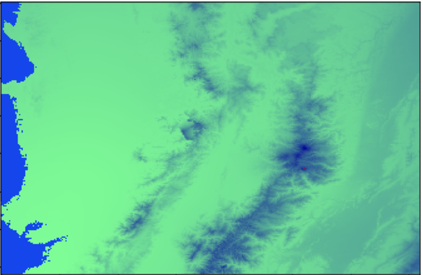
\includegraphics[scale=1]{tmax_picture_1}
	\caption{\label{tmax_picture} Mise sous forme graphique du tableau des température maximales pour le mois de janvier 2011 }
\end{figure}

\paragraph{Contexte climatique Colombien}La Colombie se trouvant à proximité de l'équateur, on y trouve que deux saisons: l'été ou saison sèche (de décembre à janvier et de juillet à août) puis l'hiver ou saison des pluies (d'avril à mai et de octobre à novembre). Le relief du pays ainsi que sa taille, font varier le climat de chaud et humide pour la partie amazonienne et la région des caraïbes, désertique pour la région de Guajira tout au nord et glacial pour les zones en haute altitude à plus de 3000 mètres. Le département de Risaralda se trouve dans le centre de la Colombie dans la région de l'Axe du café et jouit de conditions climatiques, géographiques et géologiques idéales pour la culture du café. Les températures oscillent entre 8 et 24 degrés mais un phénomène appelé \textit{El Niño} perturbe régulièrement le climat à l'échelle du continent. 

% http://www.actulatino.com/2016/01/14/colombie-el-nino-provoque-chaleur-et-secheresse-juan-manuel-santos-appelle-a-la-vigilance/

% https://public.wmo.int/fr/medias/communiqu%C3%A9s-de-presse/d%E2%80%99une-intensit%C3%A9-exceptionnelle-l%E2%80%99%C3%A9pisode-el-ni%C3%B1o-amorc%C3%A9-son-d%C3%A9clin-mais


\paragraph{El Niño}El Niño désigne un phénomène climatique qui se caractérise par une augmentation des températures de l'eau dans l'est du Pacifique sud due à une perturbation dans la circulation atmosphérique entre les pôles et l'équateur. Ces perturbations déplacent les zones de précipitations, modifient les routes des cyclones ou typhons provoquent à certains endroits de fortes précipitations et à d'autres de longues périodes de sécheresse. Même dans les zones tempérées, les périodes El Niño changent les habitudes climatiques. Durant l'été austral 2015-2016 s'est produit un des épisodes El Niño le plus fort jamais enregistré\cite{OMM}. Si une grande partie de l'Amérique du Sud a été victime de fortes précipitations, la Colombie, elle, a subit une longue période de sécheresse et l'Europe a connu des records de chaleur. Sur la figure \ref{Nino} on peut observer les différents pics correspondants à l'intensité du phénomène ainsi que pour son opposé, La Niña. 

\begin{figure}[H]
	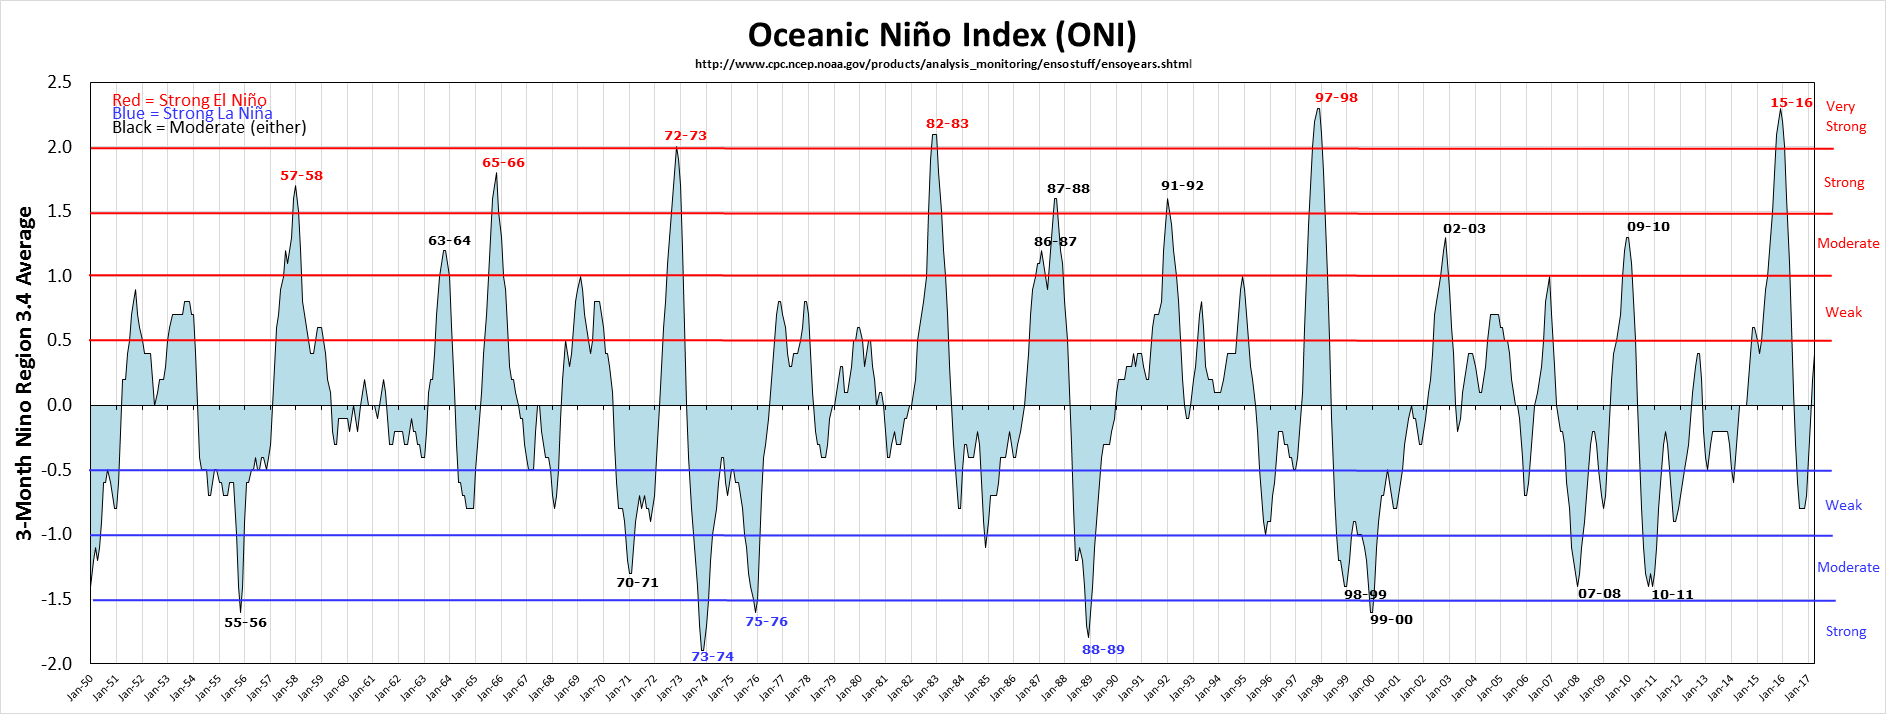
\includegraphics[scale=0.25]{VariationElNino}
	\caption{\label{Nino} Intensité du phénomène El Niño au cours des ans\newline Source: \textit{http://ggweather.com/enso/oni.htm}}
\end{figure}

\paragraph{Impact du réchauffement climatique} Outre les phases d'El Niño, il est nécessaire de rappeler que le climat mondiale se réchauffe et que des conséquences se font ressentir. Le Centre du Commerce International \cite{CCI} nous donne un aperçu des conséquences que ce réchauffement pourrait avoir pour la Colombie. "Les coûts de production sont susceptibles d'augmenter en raison des nouvelles conditions climatiques favorisant la prolifération des insectes, invasions et microbes pathogènes, et perturbant à l'équilibre naturel entre certains parasites et leurs prédateurs naturels. Les maladies se développeront vers de nouvelles zones. Les besoins en eau peuvent augmenter en raison de températures plus élevées causant plus d'évaporation, forçant de nombreux agriculteurs à recourir à l'irrigation. Dans certaines régions, les agriculteurs voudront transférer leur production de café à de plus hautes altitudes afin de chercher d'un meilleur environnement."(Guide de l'Exportateur de Café, CCI, 2011 \cite{GuideCafe})


\subsection{Données de sols} 
Les données de qualité de sol sont subdivisées en profils. Chaque profil est séparé en une ou plusieurs couches d’une certaine profondeur dont sont renseignées les caractéristiques comme le pH, la texture ou encore le taux de matière organique. Les différentes textures sont présentées sur la figure \ref{TriangleTexture}. Afin d'avoir des données uniformes, les moyennes sur les 3 premières couches jusqu'à 1 mètre de profondeur ont été réalisées pour le pH et le niveau de matière organique alors que pour la texture, la somme des variable binaire a été effectuée. \\


\noindent Les données proviennent d'un GIS (Geographical Information System), d'où il a été possible de croiser les données point par point afin d'extraire le profil de sol correspondant à un set de coordonnées GPS. Malheureusement les profils ne contiennent que pH, matière organique et texture. Des données très hétérogènes contenaient d'autres informations sur la composition chimique du sol mais leur structure et leur répartition irrégulière dans la zone de travail ont forcé à abandonner leur utilisation par manque de temps et de ressources.

% triangulo-del-suelo
\begin{figure}[H]
	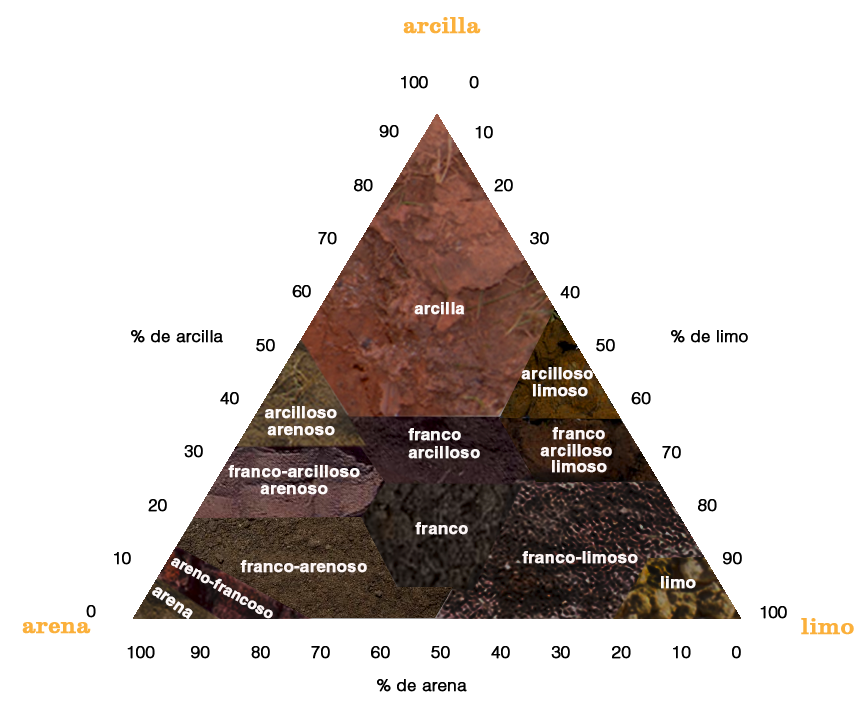
\includegraphics[scale=0.7]{triangulo-del-suelo}
	\caption{\label{TriangleTexture} Triangle représentant les différentes textures de sols\newline Source: \textit{http://www.construnatura.com/esp/articulo/agricultura-ecol-gica/el-suelo-como-fuente-de-vida--propiedades--ii-}}
\end{figure}






%################################################################################################################

\chapter{Méthodes de modélisation}
\section{Rappel des objectifs}\label{obj}
Ce projet a deux principaux objectifs. Le premier est de trouver s'il existe différents groupes de café ayant des relations entre les conditions de culture et les caractéristiques physiques ou sensorielles. On cherche donc dans cette première partie à caractériser les cafés. On peut ici parler de clustering.  Le second objectif serait de prédire les caractéristiques physiques ou sensorielles à partir des données sur les conditions de culture. Nous avons donc ici plusieurs possibilités de manières d'agir. Par exemple, si le clustering a réussi à diviser les cafés en différentes classes, on cherchera à prédire dans quelle classe se situe un nouveau café. Plus spécifiquement, on pourra se concentrer sur certains attributs du café, par exemple l'acidité, afin d'estimer quelle sera la note attribuée. 



\newpage

\section{Apprentissage supervisé}
% knn, réseaux de neurones etc
Le but de l'apprentissage supervisé est d'expliquer des sorties (outputs) à partir d'entrées (inputs). Des règles sont calculées à partir de données d'apprentissage selon différents modèles. Par la suite, le modèle est utilisé pour catégoriser des nouvelles données. On essayera ici d'expliquer les données gustatives du café ou ses défauts physiques à l'aide des données climatiques et de sols. 


\subsection{Random Forest}

La méthode Random Forest, ou \textit{forêts d'arbres décisionnels} en français, fait partie des méthodes ensemblistes\cite{EnsembleMethods}, qui utilisent la combinaison de plusieurs modèles de base, d'apprentissage automatique. Elle combine les concepts de sous-espaces aléatoires et de bagging.\\

\noindent Le bagging\label{bagging}, ou \textit{bootstrap agregation}, consiste à sous-échantillonner (ou ré-échantillonner au hasard avec doublons) le set d'entrainement et de faire générer à l’algorithme voulu un modèle pour chaque sous-échantillon. On utilise le bagging pour réduire la variance de la fonction de prédiction estimée. Le bagging semble bien fonctionner pour les procédures avec une grande variance et un petit biais, comme les arbres de décision. \cite{hastie_09_elements-of.statistical-learning}\\


\noindent Random Forest effectue donc un apprentissage sur de multiples arbres de décision entraînés sur des sous-ensembles de données légèrement différents \cite{Statistics01randomforests}.


\begin{figure}[H]
	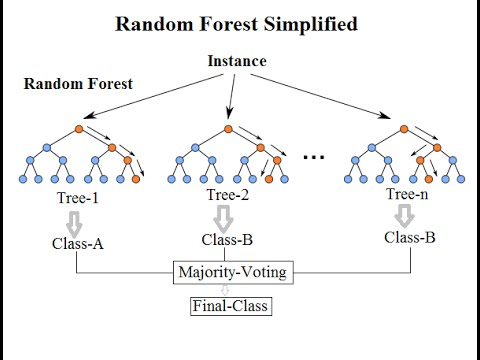
\includegraphics[scale=0.7]{RandomForestSimple}
	\caption{\label{RandomForestSchema} Schéma simple du fonctionnement de Random Forest. \newline Source: \textit{https://www.youtube.com/watch?v=ajTc5y3OqSQ}}
\end{figure}

\subsection{Partial Least Square (PLS)} 

% https://www.youtube.com/watch?v=WKEGhyFx0Dg 
% https://www.utdallas.edu/~herve/abdi-wireCS-PLS2010.pdf 

PLS, originalement pour \textit{Partial Least Squares regression} puis plus récemment pour \textit{Projection to Latent Structures} est une méthode qui combine des propriétés de la PCA ainsi que de multiples régressions linéaires. Au lieu de trouver un hyperplan de la variance maximale, entre les variables dépendantes et indépendantes, cette méthode va trouver un modèle de régression linéaire en projetant les variables indépendantes et dépendantes dans un nouvel espace. Ce sont les variables latentes. Cette méthode est particulièrement utile lorsqu'il est nécessaire de prédire un jeu de variables dépendantes à partir d'un très grand jeu de variables indépendantes.  

\begin{figure}[H] 
	\centering
	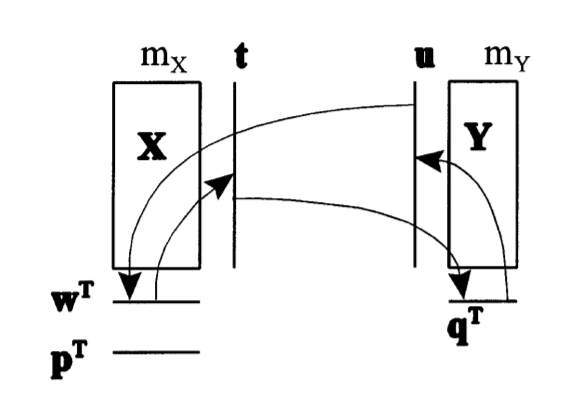
\includegraphics[scale=0.5]{PLS_1} 
	\caption{\label{PLSschema}Méthode PLS. X est représenté par son score t et Y par u. Une première estimation de U est multipliée à travers X pour obtenir une aproximation du poid $ \omega_t $. Le poid est normalisé pour être de longueur 1 et remultiplié à travers X pour produire t. A partir de t et de Y, le poid $ q^T $ est obtenu ce qui donne un nouveau vecteur u. Cette opération est répétée jusqu'à la convergence de t.\cite{CEM:CEM515}} 
	% http://www.umb.no/statisk/specmod/mbseminar/Westerhuis1998.pdf 
\end{figure} 

\subsection{Multi Block PLS} 
% http://www.models.life.ku.dk/~courses/MBtoolbox/pres_IntroMultiBlock.pdf 

% https://books.google.ch/books?id=PPUbvBUvmWoC 

% http://www.umb.no/statisk/specmod/mbseminar/Westerhuis1998.pdf 

La PLS multi block est une extension de la méthode PLS qui sépare les variables indépendantes en plusieurs blocks afin de leur donner une plus grande interpértabilité et plus d'informations sur la structure générale des données. Dans le cadre de ce projet, on peut imaginer séparer les données climatiques des données de sol par exemple.   
L'exécution est très similaire à la méthode PLS classique.  

\begin{figure}[H] 
	\centering
	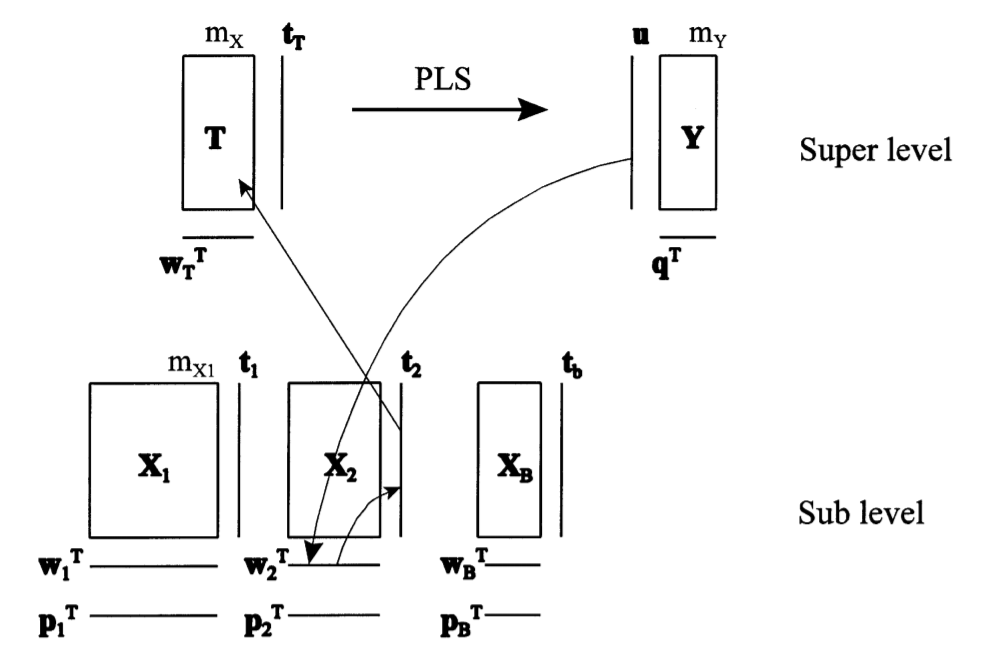
\includegraphics[scale=0.5]{MBPLS_1} 
	\caption{\label{MBPLSschema} Méthode MBPLS. Un score de départ u est régressé sur tous les blocs $ X_b $ pour donner les poids variables du bloc $ w^T_b $ Les poids des variables de blocs sont normalisés à la longueur un et multipliés par les blocs pour donner les scores de blocs $ t_b $.  Les scores de blocs sont combinés dans le super bloc T. Un cycle PLS entre T et Y est effectué pour donner le poids superieur $ W^T_T $, qui est également normalisé à la longueur un, et le super score $ t_T $. L'opération est répétée jusqu'à la convergence de $ t_T $. \cite{CEM:CEM515}} 
	% http://www.umb.no/statisk/specmod/mbseminar/Westerhuis1998.pdf 
\end{figure} 






\newpage

\section{Apprentissage non-supervisé}
Contrairement à l'apprentissage supervisé, l'apprentissage non-supervisé tente de trouver des groupes dans des données hétérogènes. Le but est d'extraire des connaissances à partir de ces données. Comme mentionné dans la partie \ref{obj}, notre but est de découvrir différents groupes de café identifiables. 


\subsection{SOM}

Les différentes classes gustatives d'un café peuvent être considérées comme des entrées afin vérifier s'il est possible de regrouper différents cafés qui se distingueraient. Afin de trouver les différentes catégories de café, nous testerons les capacités de l'algorithme SOM (pour Self Organizing Map ou Cartes Auto Adaptatives en français) qui utilise un réseau de neurones pour étudier la répartition des données dans un espace de grande dimension. 

\noindent Un bel exemple de SOM est celui de la carte de la pauvreté mondiale réalisé par le \textit{Department of Computer Science and Engineering} de l'université \textit{Helsinki University of Technology}. 

\begin{figure}[H]
	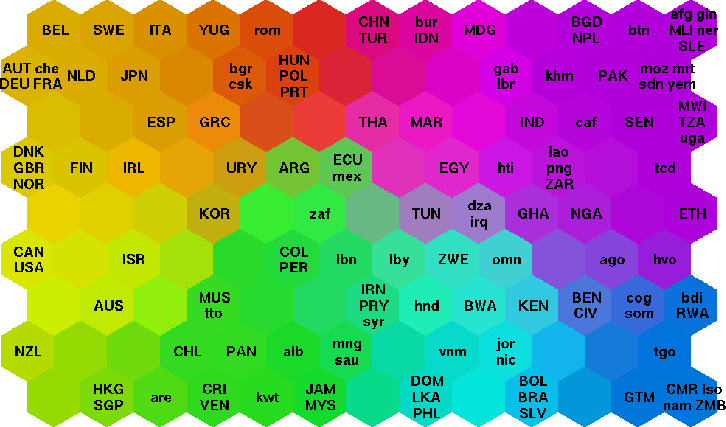
\includegraphics[scale=0.5]{SOMWordlPovertyMap}
	\caption{\label{SOMPovertyMap} Pays organisés en SOM d'après des indicateurs de pauvreté. \newline Source: \textit{http://www.cis.hut.fi/research/som-research/worldmap.html}}
\end{figure}

\begin{figure}[H]
	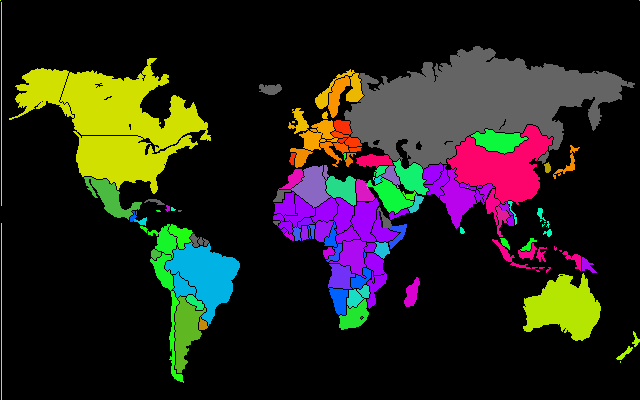
\includegraphics[scale=0.55]{worldmap}
	\caption{\label{WorldPovertyMap} Pays correspondants à la carte SOM de la figure \ref{SOMPovertyMap} \newline Source: \textit{http://www.cis.hut.fi/research/som-research/worldmap.html}}
\end{figure}




% TODO - supprimer ou pas ? c'est chiant la théorie on veut des résultats

\newpage
\section{Optimisation}

\subsection{Boosting}
Le principe du boosting est quelque peu différent du bagging (voir section \ref{bagging}). Les différents classifieurs sont pondérés de manière à ce qu’à chaque prédiction, les classificateurs ayant prédit correctement auront un poids plus fort que ceux dont la prédiction est incorrecte.\\


\noindent Adaboost est un algorithme de boosting qui s’appuie sur ce principe, avec un paramètre de mise à jour adaptatif permettant de donner plus d’importance aux valeurs difficiles à prédire, donc en boostant les classificateurs qui réussissent quand d’autres ont échoué. Des variantes permettent de l’étendre à la classification multiclasses. Adaboost s’appuie sur des classificateurs existants et cherche à leur affecter les bons poids vis à vis de leurs performances\cite{EnsembleMethods}.\\


\begin{figure}[H]
	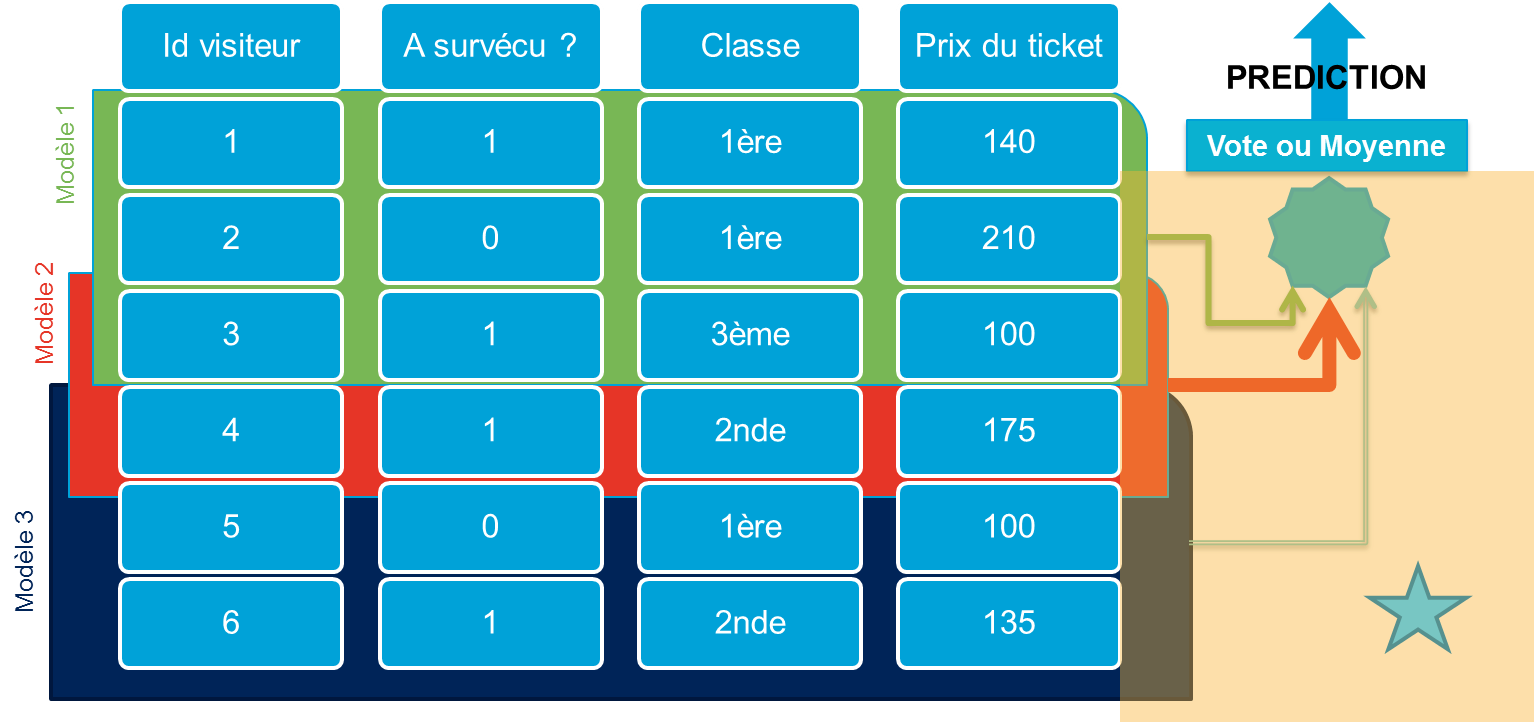
\includegraphics[scale=0.5]{boosting1}
	\caption{\label{BoostingSchema}Schéma du fonctionnement du Boosting \newline Source: \textit{http://www.cis.hut.fi/research/som-research/worldmap.html}}
\end{figure}

\noindent Gradient Boosting est une méthode de machine learning utilisée pour les problèmes de classification et de régression. Elle fait aussi partie des méthodes ensemblistes, et est utilisée majoritairement avec des arbres de décision. L'idées est encore d'agréger plusieurs classificateurs ensemble mais cette fois en les créant itérativement.\\


\noindent Le classifieur du gradient boosting est donc au final paramétré par les poids de pondération des différents mini-classifieurs, ainsi que par les paramètres des fonctions utilisées. Il s’agit donc d’explorer un espace de fonctions simples par une descente de gradient sur l’erreur\cite{EnsembleMethods}.

\subsection{Cross-Validation}

Contrairement au bagging qui est utilisé pour réduire l'overfitting en entrainant plusieurs modèles sur des données ré échantillonnées (avec répétition) puis en construisant un modèle sur la moyenne de ces modèles, la cross-validation est utilisée pour tester la fiabilité d'un modèle en se basant sur un échantillonnage des données d'entrainement et de test. Il existe plusieurs méthodes: « holdout method », « k-fold cross-validation » et « leave-one-out cross-validation ».\\

\noindent La première consiste à diviser le set de données en deux et en utilisant une partie pour entrainer le modèle puis une autre pour le tester. L'erreur est estimée en calculant un score de performance avec une méthode comme MSE (Erreur Quadratique Moyenne ou \textit{Mean Square Error}). \\

\noindent Étant donné que les données sont souvent trop peu nombreuses pour se permettre de laisser tomber dès le départ une partie des données, la k-fold cross-validation devient utile. On divise le set en k échantillons puis on en sélectionne un comme étant le set de test puis les k-1 autres comme étant le set d'entrainement. On répète l'opération en sélectionnant chaque fois un échantillon différent pour le test. Le score de performance est calculé en réalisant la moyenne des scores des k validations effectuées. La méthode « Leave-one out » utilise le même principe mais en ne laissant qu'une seule entrée en dehors du set d'entrainement à chaque tour\cite{hastie_09_elements-of.statistical-learning}. 



	
	
\chapter{Analyse des données}
\minitoc

\newpage
\section{Data Mining - Analyse exploratoire}

\subsection{Pré-traitement}
%Description du dataset (rapidement, le reste dans un codebook)\\

%Mise en forme du dataset, une sortie à la fois vs plusieurs sorties etc \\
%On considère les données gustatives et les défauts physiques comme des sorties -> les prendre un par un ou tous ensemble\\

%Description du set, différentes parties des données, éventuelles données manquantes\\

Une grande partie de l'étape de pré-traitement a été réalisée durant l'extraction des données. Il a en effet fallu les extraire d'une manière uniforme et cohérente dès le départ afin de ne pas se retrouver avec des variables présentes uniquement dans certaines parties du set de données ou avec des variables incohérentes comme cela a été le cas de certains cafés qui avaient comme note de dégustation plus de cent points sur cent par exemple. Des éliminations ou des corrections ont été réalisées de manière automatisées et manuelles afin de supprimer les erreurs. On notera parmi les corrections importantes le remplacement de virgules par des points, quelques erreurs de frappes (68.5 points sur 10 au lieu de 6.85 par exemple) ou encore des utilisations d'unités différentes selon les sources. Le dataset résultant est décrit dans l'Annexe A de ce projet. Une fois cette étape de d'extraction et de nettoyage réalisée, les premières informations ont pu être extraites des données.\\


\noindent Le schéma \ref{DatasetMaking} résume rapidement les différentes éliminations d'observations au cours des étapes de construction du set de données. 

\begin{figure}[H]
	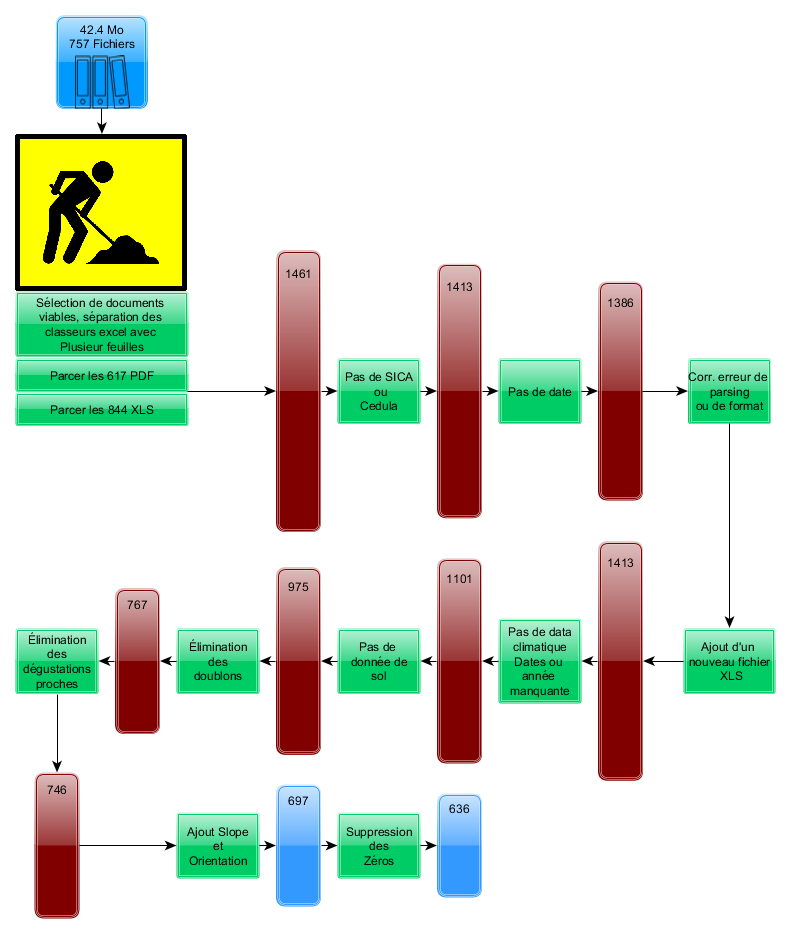
\includegraphics[scale=0.5]{Dataset_2}
	\caption{\label{DatasetMaking} Étape de construction du set de données et pertes d'observations.}
\end{figure}



\paragraph{Variables dépendantes\label{VarDep}} Les variables de sorties, ou dépendantes, sont composées des dix analyses de dégustation et éventuellement de la totalité des défauts physiques des grains. Sauf pour les défauts physiques des grains, qui sont éliminés avant la dégustation, les variables de sorties sont très corrélées entre elles et il a été discuté avec le responsable du comité des caféiculteurs de Risaralda, M. Felipe Rincón, de sélectionner les variables les plus importantes. Ces variables sont \textit{Acidez}, \textit{Dulzor} et \textit{Puntaje Total} ainsi que la catégorie décrite dans le paragraphe suivant qui a été ajouté au set de données.  

\paragraph{Catégories}
Les cafés colombiens sont réputés excellents mais sur les 100 points attribuable lors des dégustations qu'est-ce que cela représente ? Le tableau \ref{categoriesCafe} nous donne une bonne idée de l'échelle de notation. Ces catégories seront utilisées dans le set de données pour tenter de réaliser une classification. 
\begin{table}[H]
	\centering
	\caption{Catégories de cafés d'après le nombre de points \newline Source: http://www.scaa.org/?page=resources\&d=cupping-protocols \label{categoriesCafe}}
	\begin{tabular}{llllcl}
		\textbf{Total Score}   &  & \textbf{Quality Classification}   & \textbf{Specialty or not}  & \textbf{Category} \\
		
		90-100        &  & Outstanding              & Specialty         &  1                    \\
		85-89.99      &  & Excellent                & Specialty         &  2                    \\
		80-84.99      &  & Very Good                & Specialty         &  3                    \\
		\textless80.0 &  & Below Specialty Quality & Not Specialty     &  4                   
	\end{tabular}
\end{table}



\paragraph{Élimination des résultats avec zéro points} Certain cafés du dataset ont zéro points en sortie pour chacune des 10 catégories notées. Il a été décidé de ne pas prendre en compte ces cafés lors des calculs de prédiction ou de clustering car la qualité du sol ou du climat ne peut justifier une telle baisse de qualité à elle seule dans une région réputée propice et qu'un défaut de traitement du grain, un mauvais tri avant la dégustation ou autre facteur externe doit en être la cause. Cependant, afin de se faire une idée d'éventuelles causes de cette qualité médiocre, les cafés sus-mentionnés ont été gardés pour la réalisation des cartes SOM au chapitre \ref{SOM}. 





\subsection{Analyse exploratoire et apprentissage non-supervisé}

\subsubsection{Corrélations entre variables}

Afin d'avoir une bonne vue d'ensemble sur les variables et leurs liens, les matrices de corrélation ont été calculées pour toutes les variables. Premièrement la corrélation entre les différentes sorties. Sur la figure \ref{correlation_sorties1} on peut observer que les défauts physiques des grains ne sont que très peu liés entre eux ou avec les résultats de dégustation. On remarque cependant que les données gustatives du café sont fortement liées entre elles. 

\begin{figure}[H]
	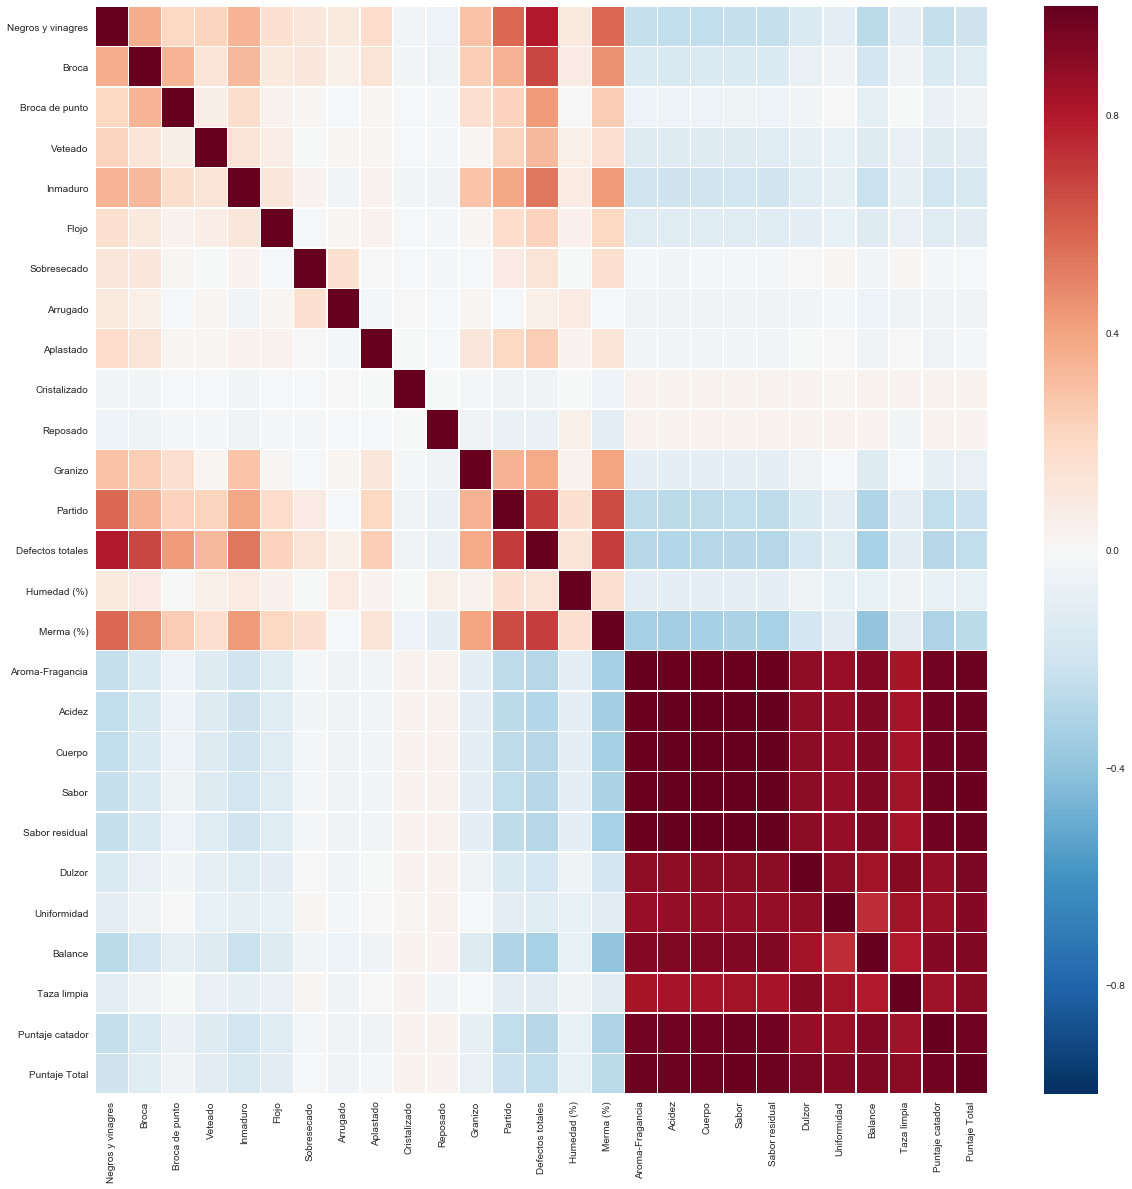
\includegraphics[scale=0.35]{correlation_sorties1}
	\caption{\label{correlation_sorties1} Matrice de corrélation entre les différentes sorties.}
\end{figure}


\noindent Sur la figure \ref{correlation_all1} on peut observer les corrélations entre toutes les variables. 


\begin{figure}[H]
	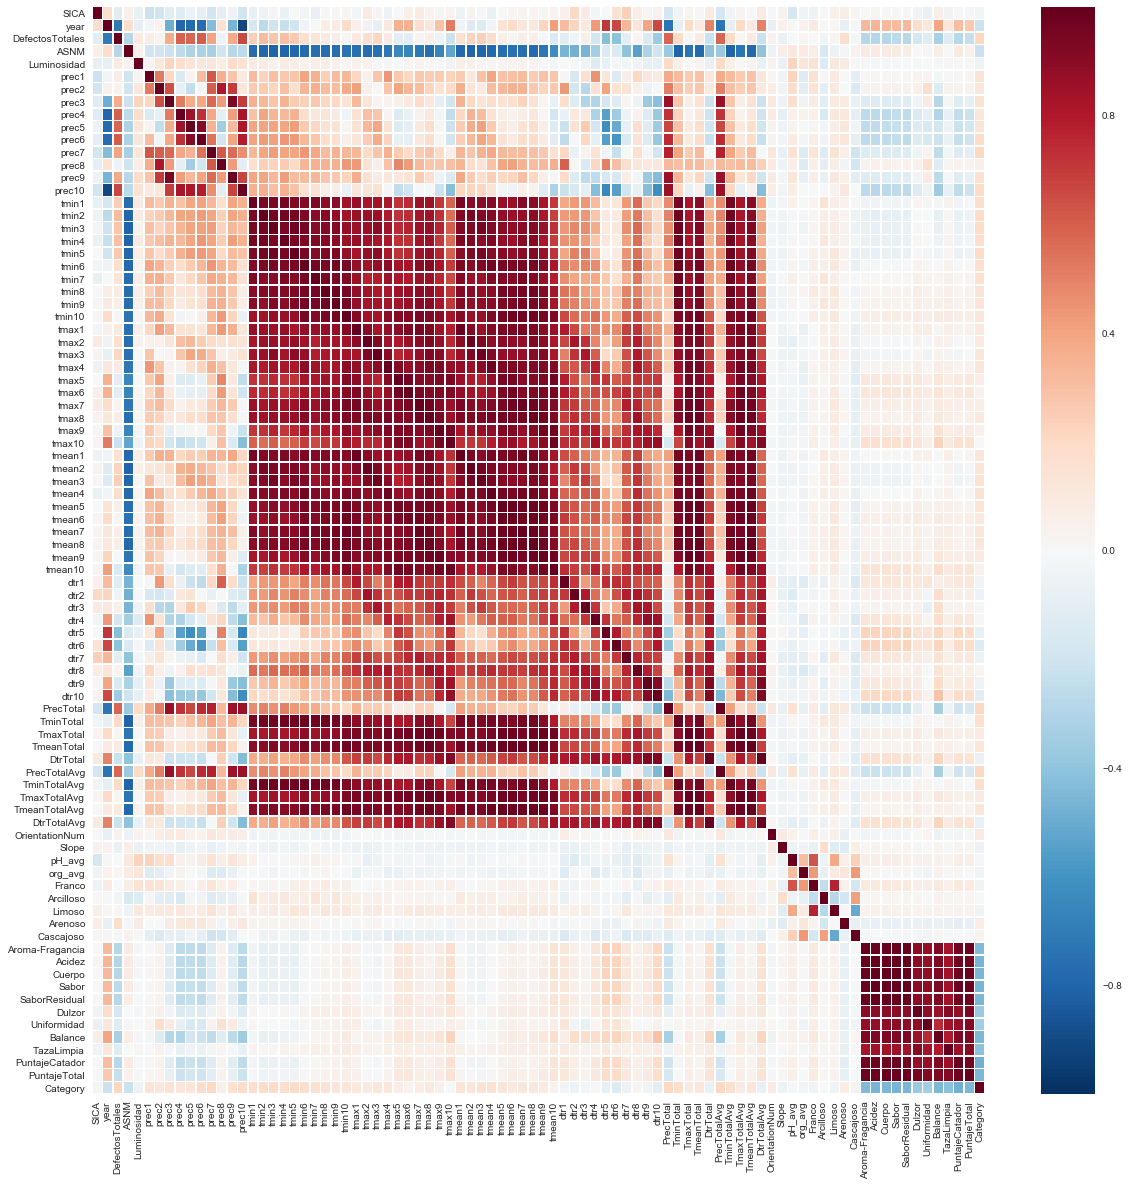
\includegraphics[scale=0.35]{correlation_all1}
	\caption{\label{correlation_all1} Matrice de corrélation entre toutes les variables.}
\end{figure}


\noindent On observe que les données de sol sont parfois corrélées entre-elles mais presque pas du tout avec les données climatiques. On peut donc déjà soulever que le climat n'a pas ou peu d'influence sur la texture, le pH ou le taux de matière organique du sol des zones étudiées. Les précipitations ont une influence importante sur les défauts physiques des grains, en revanche nous n'avons aucune variable qui a une corrélation marquée avec les points totaux et donc la qualité du café.   



%TODO Parler des variétés de cafés et de quelques données les concernants (Moyennes de points, rendement par variété, altitude etc) 
%TODO afficher des moyennes par année etc



\newpage
\subsubsection{Principal Component Analysis (PCA)}\label{PCAss}
La PCA, pour Analyse en Composantes Principales en français, est une méthode qui consiste à transformer un jeu de variables corrélées en nouvelles variables dé-corrélées les unes des autres. Ces nouvelles variables sont appelées composantes principales et permettent de rendre l'information moins redondante. Pour faire plus simple, l'utilité de la Composante Principale est de réduire le nombre de variables tout en gardant un maximum d'information. La figure \ref{PCAdefinition} montre une représentation graphique de la composante principale. 


\begin{figure}[H]
	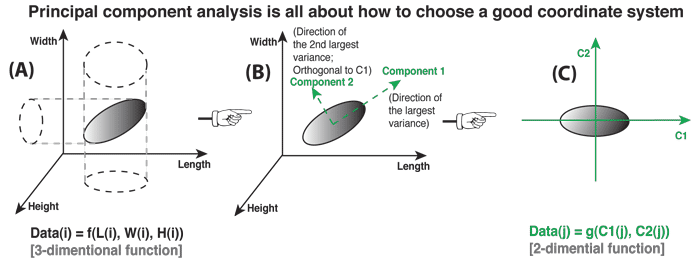
\includegraphics[scale=0.5]{PCA_1}
	\caption{\label{PCAdefinition} Description de l'Analyse en Composante Principale. (A) Description d'un objet simple de manière compliquée ( trois dimensions pour par exemple une ellipse en papier) (B) Trouver des nouvelles variables (axes de coordonnées) orthogonaux l'un à l'autre qui pointent dans les directions de la plus grande variance (C) Utiliser les nouvelles variables (axes) pour décrire l'objet d'une manière plus simple. }
\end{figure}

\paragraph{Résultats de la PCA}

L'analyse sur une version compacte des variables a donné les résultats présentés dans le tableau \ref{TablePCAResult1} et sur la figure \ref{FigurePCAResult1}. Une première analyse avait été effectuée sur le set de données complet, c'est-à-dire avec la totalité des données climatiques et non les moyennes, et les résultats se sont avérés similaires mais plus difficilement lisibles. Il a donc été choisi de résumer les variables pour réaliser la PCA et le clustering. La PCA du tableau \ref{TablePCAResult1} ne comprend pas les cafés avec zéro points.
\begin{table}[]
	\centering
	\begin{tabular}{lllllll}
		& PC1     & PC2     & PC3     & PC4     & PC5     & PC6     \\
		ASNM           & \textbf{0.4125}  & 0.0766  & -0.0360 & 0.1766  & -0.1337 & 0.0397  \\
		Luminosidad    & -0.0169 & 0.2320  & 0.1532  & -0.3178 & -0.2836 & 0.0157  \\
		PrecTotalAvg   & -0.1714 & 0.1424  & 0.0222  & \textbf{-0.6767} & -0.0667 & 0.0926  \\
		TminTotalAvg   & \textbf{-0.4589} & -0.0115 & 0.1086  & -0.1232 & 0.0013  & 0.0809  \\
		TmaxTotalAvg   & \textbf{-0.4745} & -0.0334 & 0.0296  & 0.1501  & -0.0253 & -0.0329 \\
		TmeanTotalAvg  & \textbf{-0.4803} & -0.0252 & 0.0631  & 0.0409  & -0.0149 & 0.0133  \\
		DtrTotalAvg    & -0.3323 & -0.0517 & -0.0884 & \textbf{0.4712}  & -0.0529 & -0.1769 \\
		OrientationNum & 0.0623  & 0.0592  & -0.0886 & -0.1839 & \textbf{0.3797}  & \textbf{-0.5662} \\
		Slope          & 0.0657  & -0.1842 & 0.1179  & 0.1047  & 0.0434  & \textbf{0.6905}  \\
		pH\_avg        & 0.0135  & 0.3892  & 0.3844  & -0.0168 & 0.1244  & 0.0679  \\
		org\_avg       & 0.0493  & 0.1781  & \textbf{0.5036}  & 0.2176  & -0.1639 & -0.1841 \\
		Franco         & -0.0157 & \textbf{0.5453}  & 0.1441  & 0.1921  & 0.1676  & 0.1108  \\
		Arcilloso      & -0.0180 & -0.3026 & 0.2993  & -0.0844 & \textbf{0.4532}  & 0.1751  \\
		Limoso         & -0.0754 & \textbf{0.5018}  & \textbf{-0.2016} & 0.1095  & 0.2726  & 0.1712  \\
		Arenoso        & -0.0210 & 0.0645  & 0.0180  & 0.0048  & \textbf{-0.6303} & -0.0156 \\
		Cascajoso      & 0.0760  & -0.2236 & \textbf{0.6130}  & 0.0095  & 0.0109  & \textbf{-0.2053}
	\end{tabular}
	\caption{\label{TablePCAResult1}Tableau des rotations des six premiers composants de la PCA avec mise en évidence des variables les plus importantes par composante.}
\end{table}


\begin{figure}[H]
	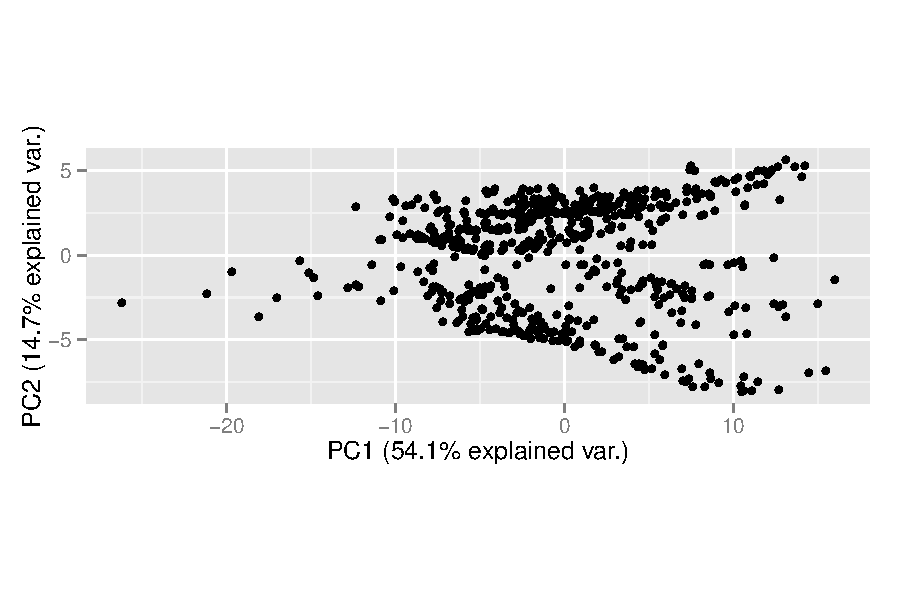
\includegraphics[scale=1]{pca_complete.pdf}
	\caption{\label{FigurePCAResult1} Résultats de la PCA sous forme graphique. Réalisé avec la totalité des variables }
\end{figure}


\paragraph{Analyse des composantes} Le tableaux \ref{TablePCAResult1} montre l'importance des variables dans les différentes composantes de la PCA réalisée avec un  jeu de variables simplifié pour plus de lisibilité, après vérification que l'importance des types de variables des deux tableaux était similaire. \\

\noindent La première composante met en évidence les températures par rapport à l'altitude alors que la deuxième et la troisième mettent en évidence principalement les caractéristiques du sol. La quatrième montre une dé-corrélation entre les précipitations moyennes et les DTR et la cinquième composante montre une corrélation entre la texture argileuse du sol et son orientation à l'opposé à d'un sol sablonneux. La sixième composante met en évidence une relation entre l'orientation et et les sols rocailleux à l'opposé des sols pentus. 


\paragraph{PCA avec prcomp} Afin de visualiser au mieux les données dans la PCA, une autre PCA a été réalisée àl'aide d'un autre outil (prcomp) et chaque point a été coloré selon son année (figure \ref{fig:pcayear}) ou selon sa catégorie (figure \ref{fig:pcacat}). 


\begin{figure}[H]
	\centering
	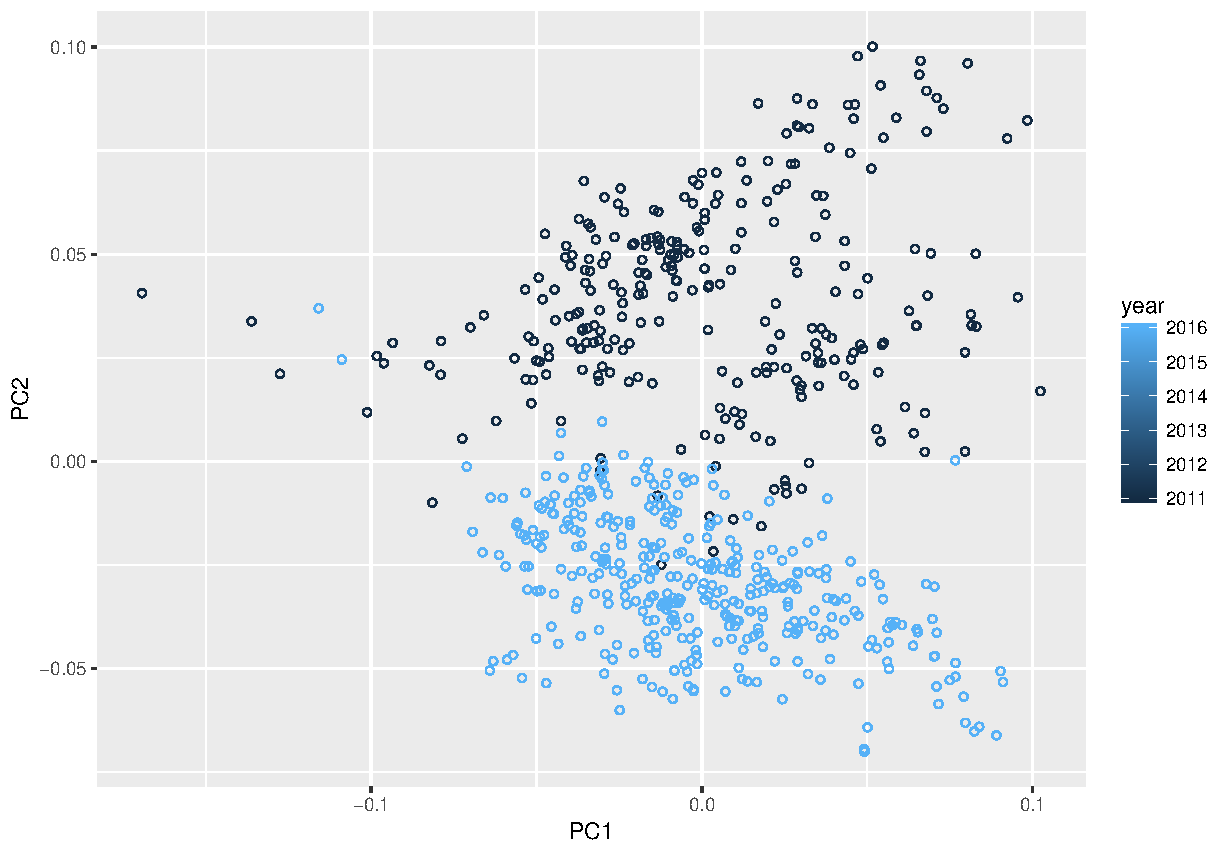
\includegraphics[width=0.7\linewidth]{img/PCA/PCAYear}
	\caption{PCA avec Prcomp: Coloration par année}
	\label{fig:pcayear}
\end{figure}


\begin{figure}[H]
	\centering
	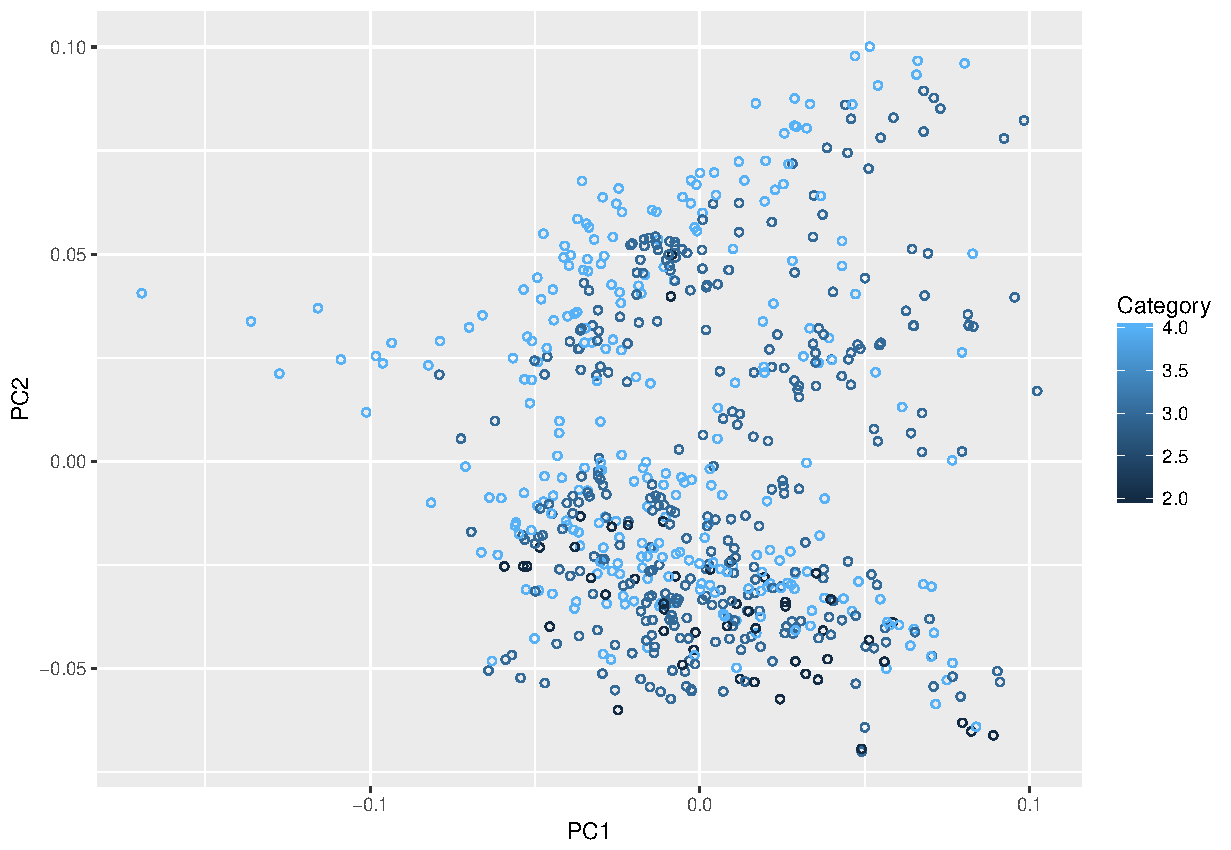
\includegraphics[width=0.7\linewidth]{img/PCA/PCACat}
	\caption{PCA avec Prcomp: Coloration par catégorie}
	\label{fig:pcacat}
\end{figure}





\noindent On peut observer que les deux années sont bien différenciées. Les premiers composants de la PCA montrent l'importance des variables climatiques et les différences entre années sont visibles sur ces graphiques. Les catégories sont aussi différemment réparties. En retournant sur les moyennes de chaque année (Voir description des données section \ref{YearlyPuntajeTotal}), on peut voir que l'année 2011 possède en effet moins de café en nombre mais plus de cafés ayant reçu la note de zéro. On peut aussi voir que les conditions climatiques sont différentes entre les deux années, surtout en termes de précipitations. La section \ref{SOM} montre les relations entre le climat et les défauts totaux, qui peuvent influencer la qualité finale du café.  %TODO
% https://georgemdallas.wordpress.com/2013/10/30/principal-component-analysis-4-dummies-eigenvectors-eigenvalues-and-dimension-reduction/

%https://onlinecourses.science.psu.edu/stat505/node/54
\newpage
\subsubsection{Clustering} Afin de vérifier la présence éventuelle de groupes d'individus parmi la population de café, nous réalisons un HCPC, pour \textit{Hierarchical Clustering on Principal Components}, à l'aide de la PCA. La figure \ref{HCTSuggest} nous montre l'arbre hiérarchique créé ainsi que le nombre de cluster proposé. \\

\begin{figure}[H]
	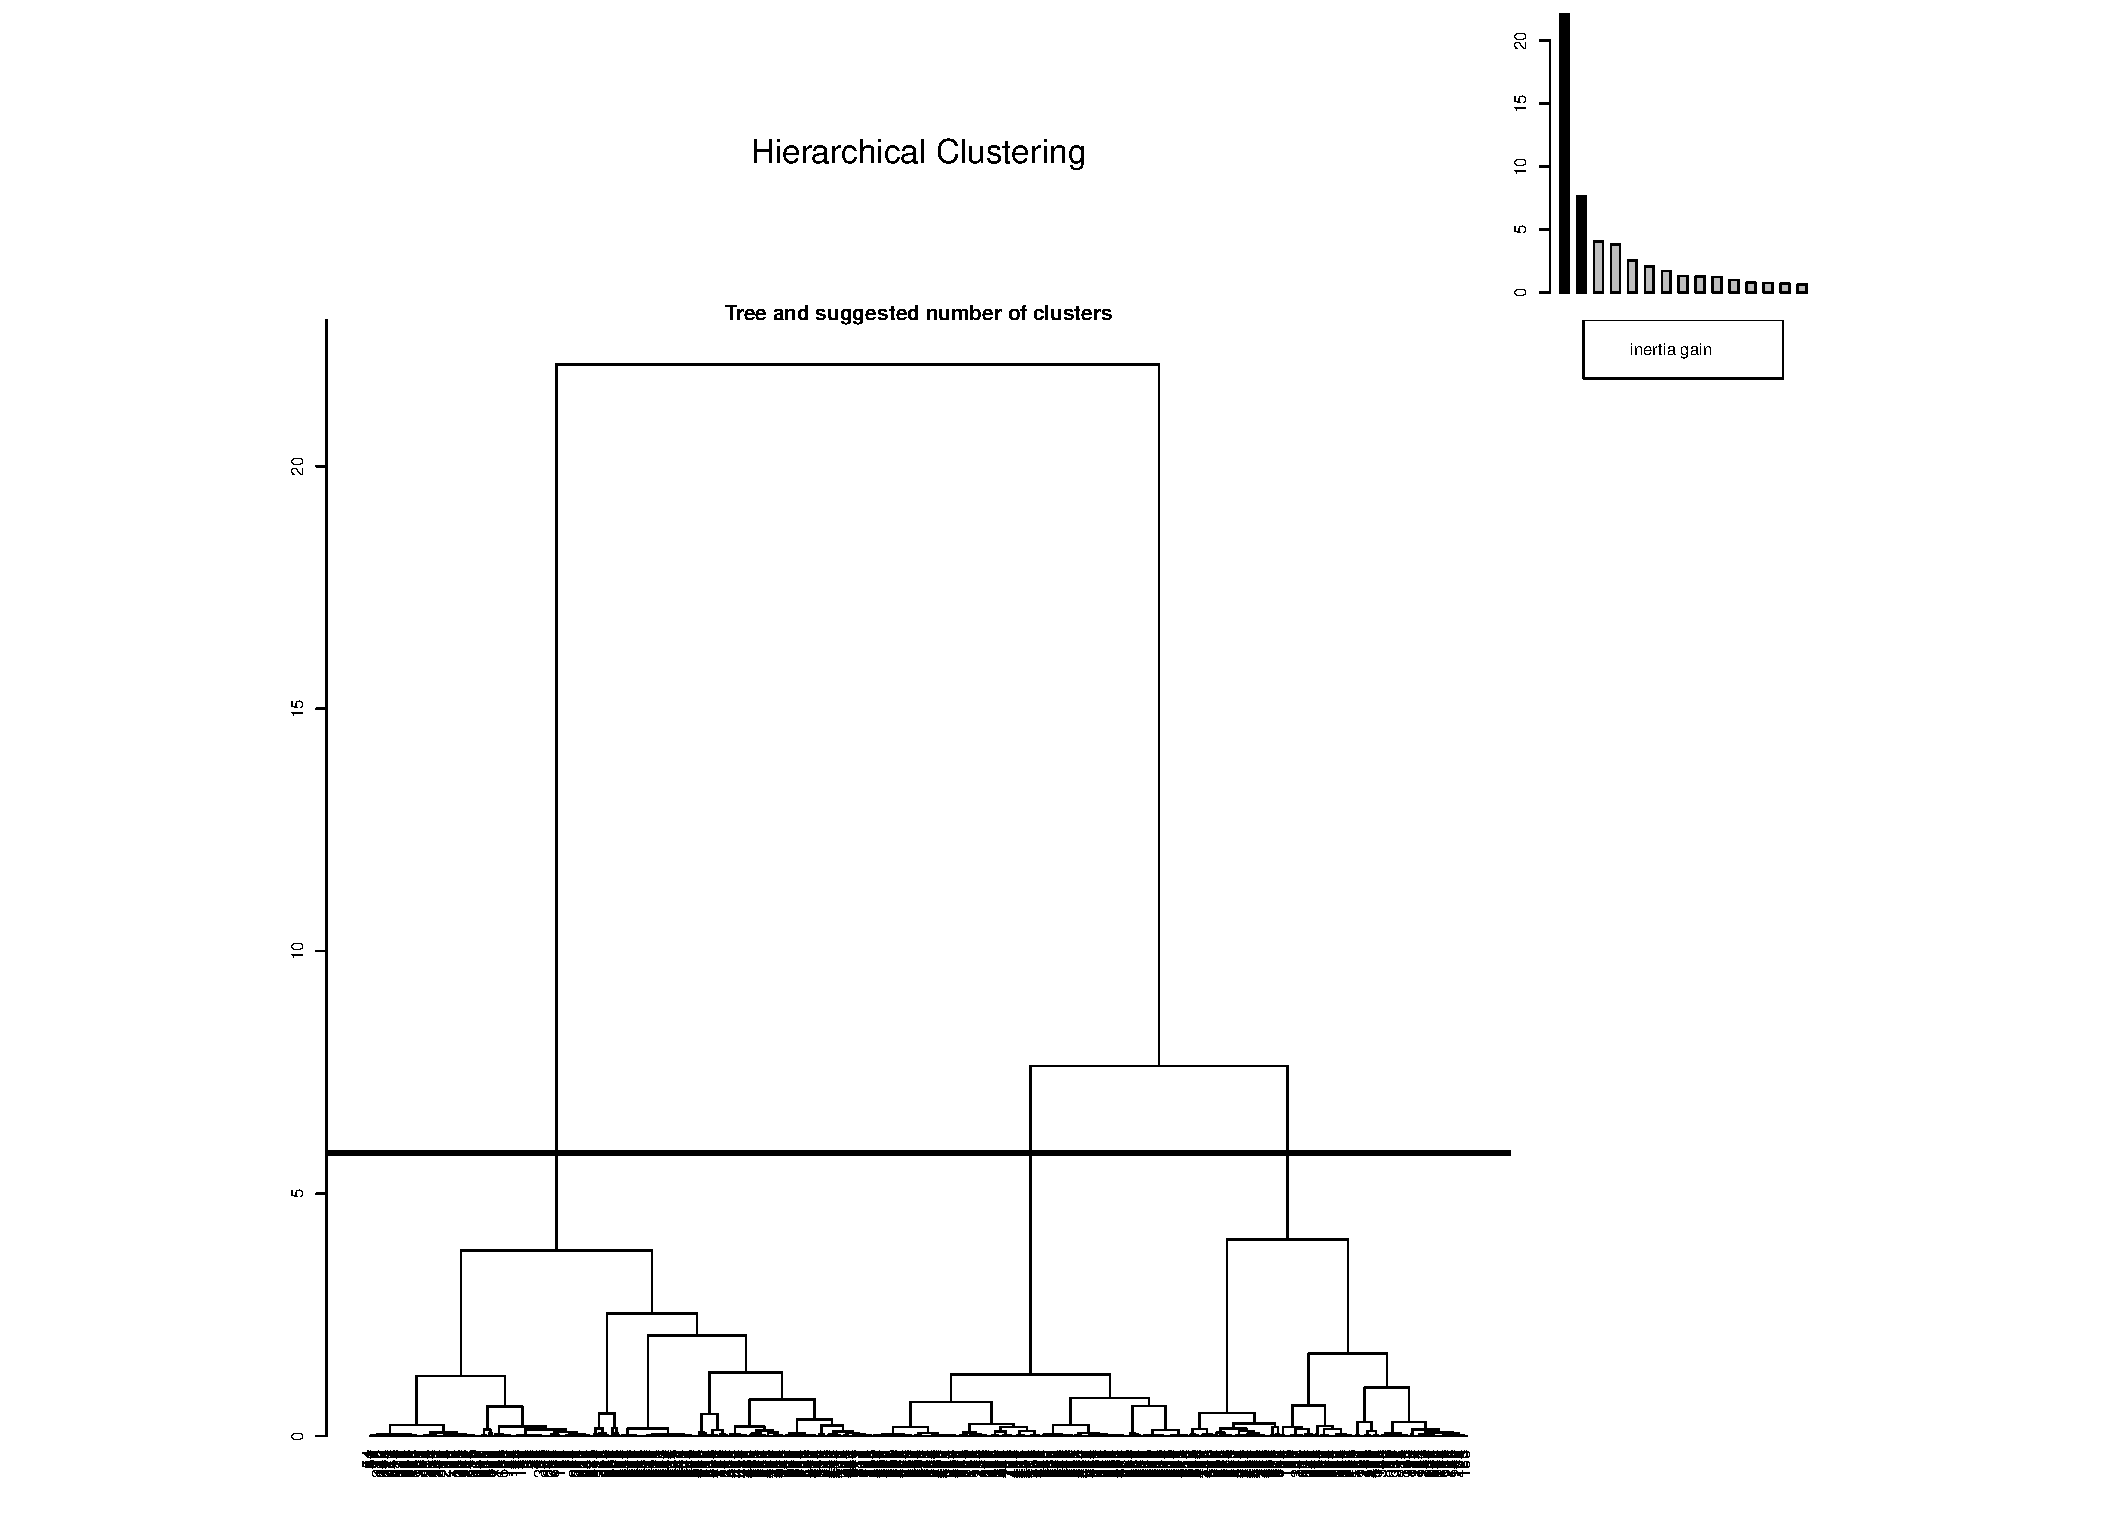
\includegraphics[scale=0.45]{HierarchicalClustering_TreeAndSuggestedNbCluster.pdf}
	\caption{\label{HCTSuggest} HCPC et proposition de nombre de cluster }
\end{figure}

\noindent La figure \ref{HCT_3d} montre une représentation du HCPC en 3D. On reconnais la forme de la PCA mais les clusters sont plutôt décevants car le découpage je fais pas ressortir les groupes éventuellement visibles. Comme on l'a vu précédemment, avec la PCA et les différentes moyennes, les deux années sont très différentes et on aurait pu s'attendre à un clustering plus efficace. 

\begin{figure}[H]
	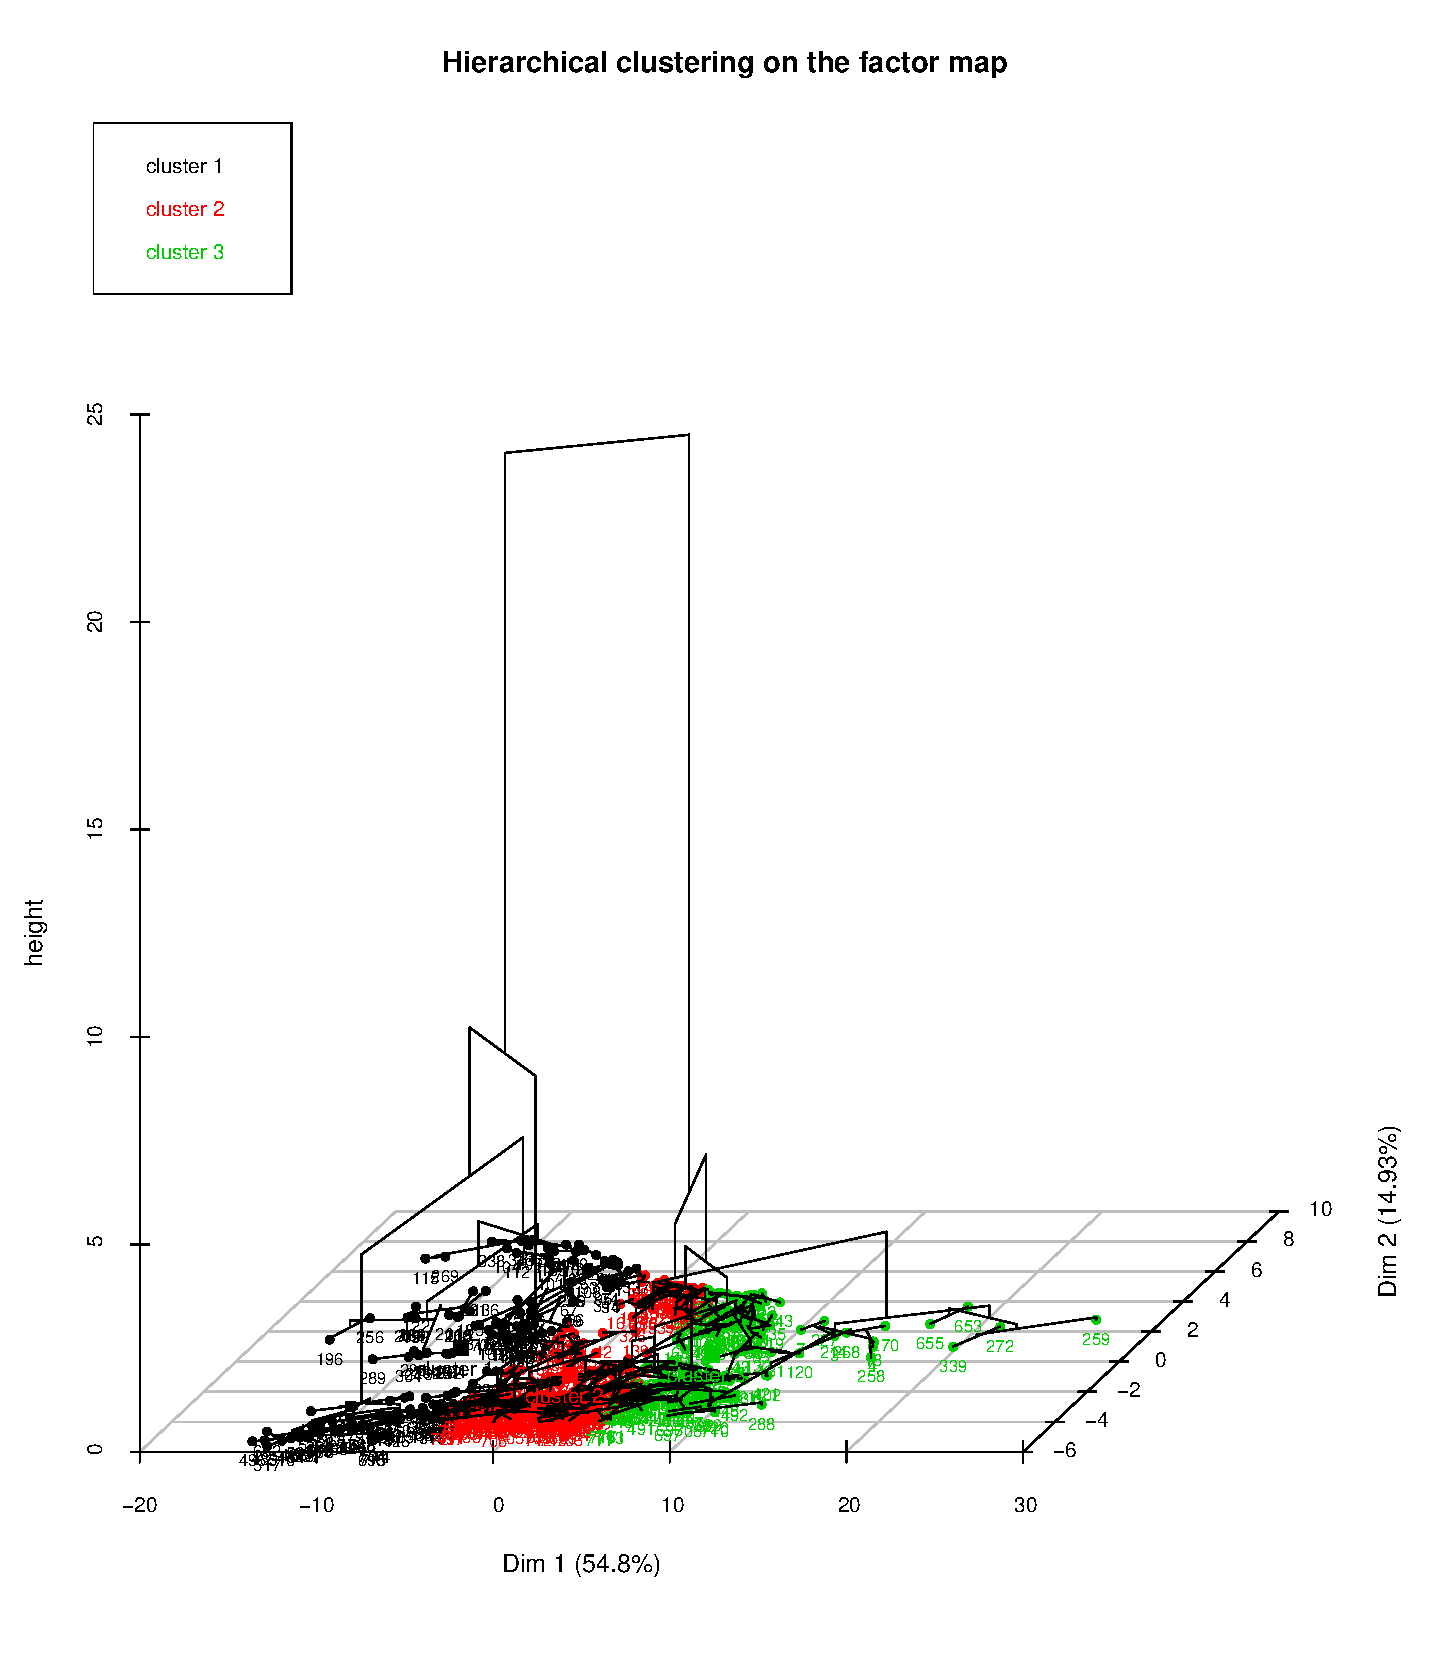
\includegraphics[scale=0.6]{HierarchicalClustering3D.pdf}
	\caption{\label{HCT_3d} HCPC arbre 3D}
\end{figure}


\noindent La figure \ref{HCT_Inert} nous montre les sauts d'inertie du dendogramme. On peut y voir qu'entre 2 et 3 clusters nous avons un saut assez grand puis à nouveau entre 4 et 5 avant une stabilisation. 


%http://www.sthda.com/english/wiki/hcpc-hierarchical-clustering-on-principal-components-hybrid-approach-2-2-unsupervised-machine-learning

\begin{figure}[H]
	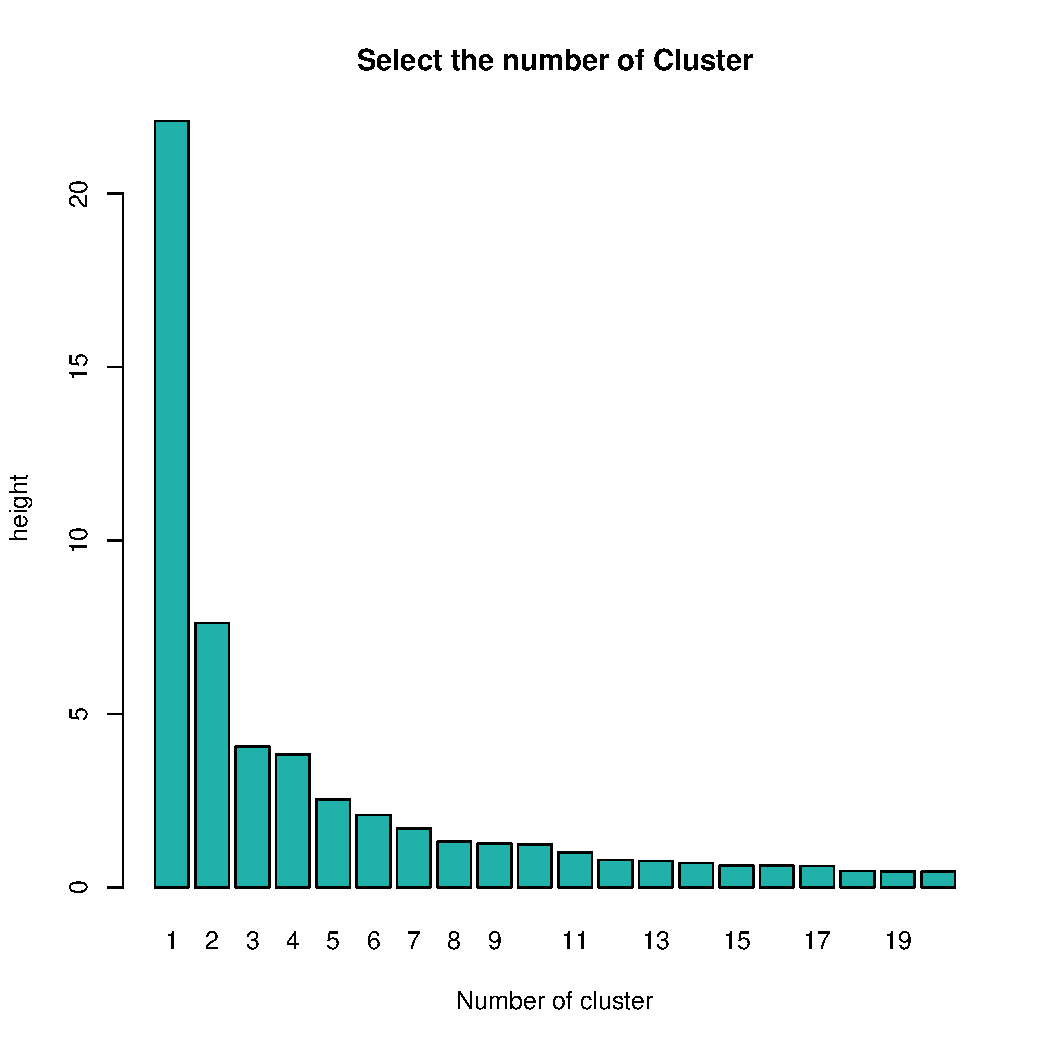
\includegraphics[scale=0.55]{NbClusterSelectInertiaGain.pdf}
	\caption{\label{HCT_Inert} Saut d'inertie du dendogramme  }
\end{figure}

%\noindent L'outil de HCPC nous fournit en sortie un objet de description des classes par les variables





\noindent L'ajout de clusters au set de données serait utile du moment que les clusters permettent significativement de séparer les types de cafés, au sens variables dépendantes du terme. Visuellement on devrait pouvoir observer une différence entre le nombre de café dans chaque cluster et les variables de sorties. Cependant ce n'est pas le cas comme on peut le voir ci-dessous: 


\begin{table}[H]
	\centering
	\label{cluster3category}
	\begin{tabular}{llll}
		 & 1  & 2  & 3   \\
		 \hline
		cat 2            & 0  & 28 & 21  \\
		cat 3            & 72 & 98 & 146 \\
		cat 4            & 44 & 70 & 157 
	\end{tabular}
	\caption{HCPC avec trois clusters comparés à la sortie catégories}
\end{table}


\noindent Les autres résultats ainsi que l'importance des variables pour la génération des clusters se trouvent dans l'annexe \ref{annexe:clust}.\\


\noindent Les variables participent presque toute activement à la séparation en partie (en prenant en compte les 5\% de probabilité critiques ) cependant la séparation n'apporte rien au set de donnée puis-qu'elle ne sépare en rien les différents types de cafés (note basse - note haute).



%\paragraph{Analyse des résultats de clustering}
%TODO - vérifier






















\newpage
\subsubsection{Self-Organizing Map}\label{SOM}
%TODO 

\paragraph{U-Matrix, répartition des cafés par classes et composants} 
La carte auto-organisatrice a été réalisée en incluant toutes les variables afin de voir où se placent les variables dépendantes par rapport aux variables indépendantes et de permettre d'observer d'éventuels clusters. 


\begin{figure}[H]
	\centering
	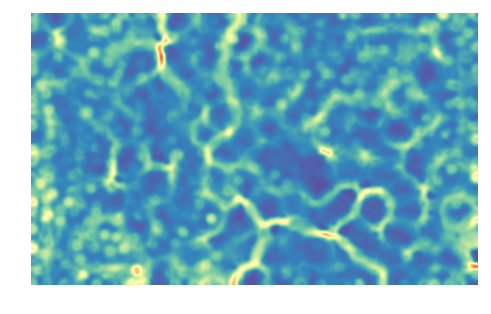
\includegraphics[width=0.7\linewidth]{SOM/SOM_Umatrix}
	\caption{U-Matrix de la carte SOM}
	\label{}
\end{figure}

\begin{figure}[H]
	\centering
	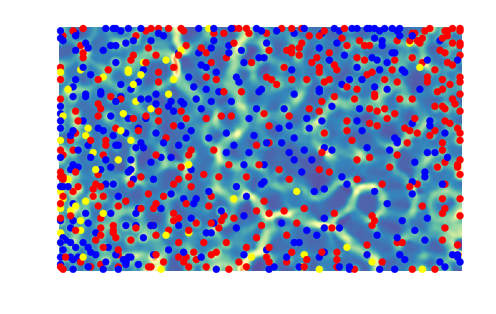
\includegraphics[width=1\linewidth]{SOM/SOM_Umatrix_Points_Category}
	\caption{\label{umatrix_cat}U-Matrix avec les points. En jaune les cafés de catégorie 2,en bleu catégorie 3 et en rouge catégorie 4. Les catégories sont expliquées au point \ref{EmpFermes}}
	\label{}
\end{figure}


\begin{figure}[H]
	\caption{Composants de qualité - Variables de sortie}
	\centering
		\subfloat[Acidez]{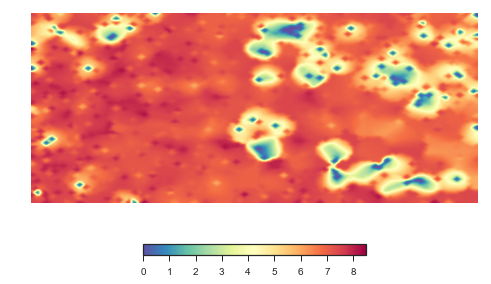
\includegraphics[width=.3\linewidth]{SOM/SOM_Acidez}}\hfill
		\subfloat[Aroma-Fragrancia]{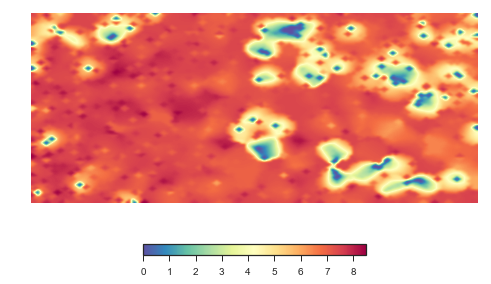
\includegraphics[width=.3\linewidth]{SOM/SOM_AromaFragrancia}}\hfill
		\subfloat[Cuerpo]{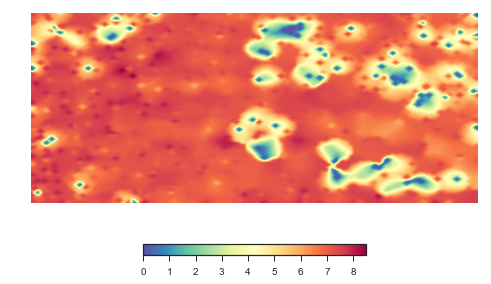
\includegraphics[width=.3\linewidth]{SOM/SOM_Cuerpo}}
		\newline
		\subfloat[Balance]{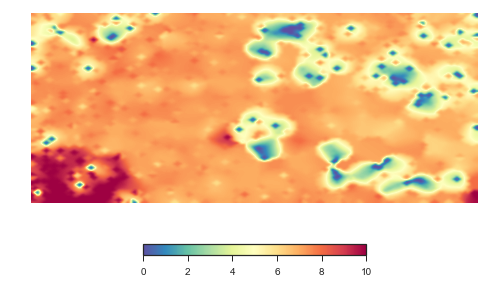
\includegraphics[width=.3\linewidth]{SOM/SOM_Balance}}\hfill
		\subfloat[Uniformidad]{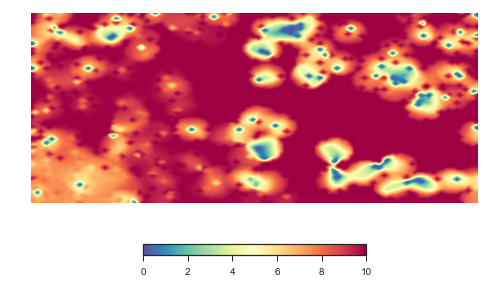
\includegraphics[width=.3\linewidth]{SOM/SOM_Uniformidad}}\hfill
		\subfloat[Taza Limpia]{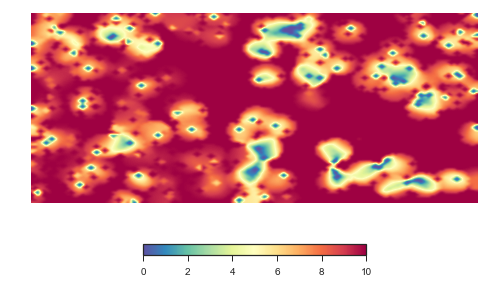
\includegraphics[width=.3\linewidth]{SOM/SOM_TazaLimpia}}
		\newline
		\subfloat[Dulzor]{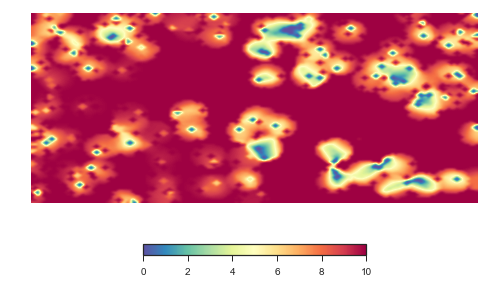
\includegraphics[width=.3\linewidth]{SOM/SOM_Dulzor}}\hfill
		\subfloat[Sabor]{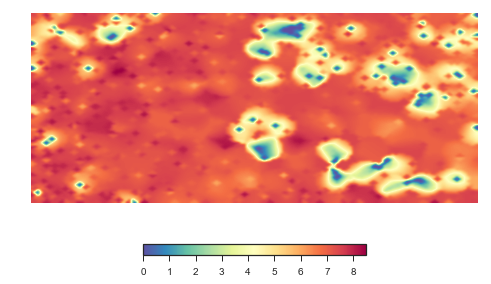
\includegraphics[width=.3\linewidth]{SOM/SOM_Sabor}}\hfill
		\subfloat[Sabor Residual]{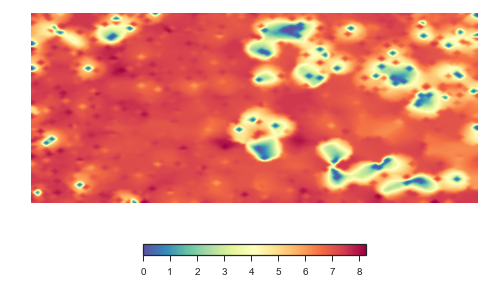
\includegraphics[width=.3\linewidth]{SOM/SOM_SaborResidual}}
		\newline
		\centering
		\subfloat[Puntaje Catador]{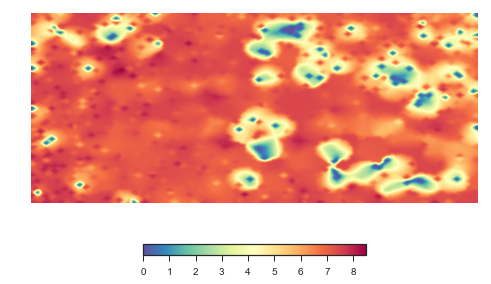
\includegraphics[width=.3\linewidth]{SOM/SOM_PuntajeCatador}}\hfill
		\subfloat[Puntaje Total]{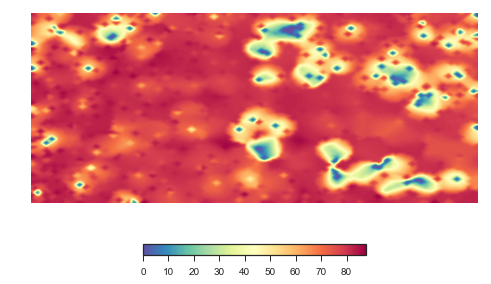
\includegraphics[width=.3\linewidth]{SOM/SOM_PuntajeTotal}}
\end{figure}




\begin{figure}[H]
	\caption{Précipitations}
	\centering
	\subfloat[Prec1]{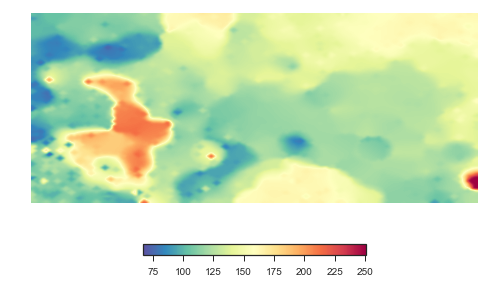
\includegraphics[width=.3\linewidth]{SOM/SOM_Prec1}}\hfill
	\subfloat[Prec2]{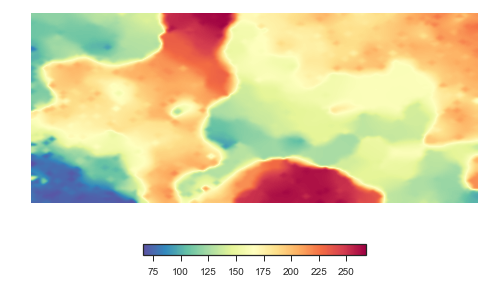
\includegraphics[width=.3\linewidth]{SOM/SOM_Prec2}}\hfill
	\subfloat[Prec3]{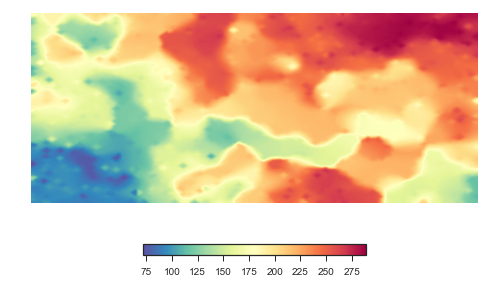
\includegraphics[width=.3\linewidth]{SOM/SOM_Prec3}}\hfill
	\newline
	\subfloat[Prec4]{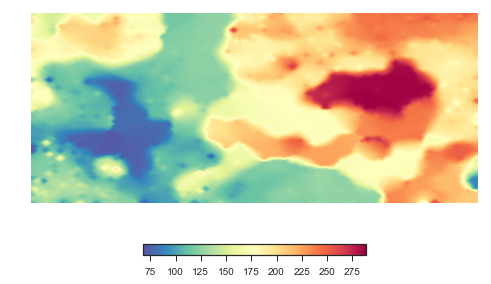
\includegraphics[width=.3\linewidth]{SOM/SOM_Prec4}}\hfill
	\subfloat[Prec5]{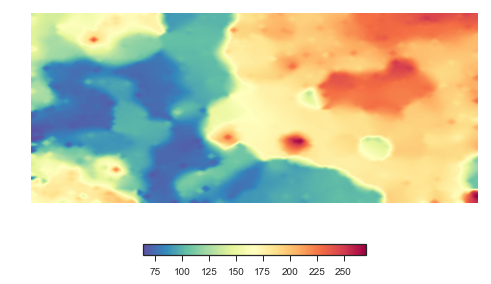
\includegraphics[width=.3\linewidth]{SOM/SOM_Prec5}}\hfill
	\subfloat[Prec6]{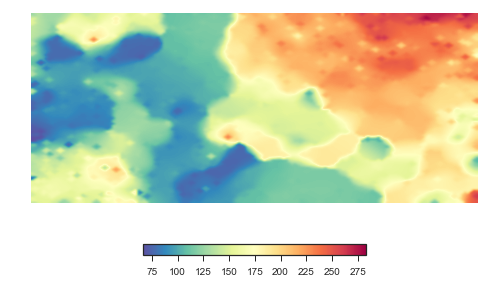
\includegraphics[width=.3\linewidth]{SOM/SOM_Prec6}}\hfill
	\newline
	\subfloat[Prec7]{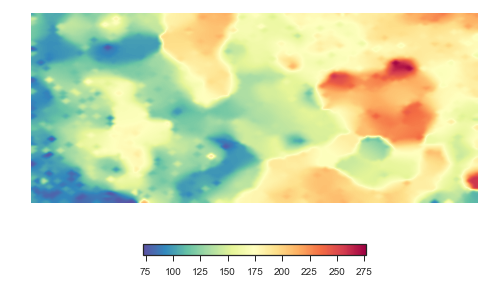
\includegraphics[width=.3\linewidth]{SOM/SOM_Prec7}}\hfill
	\subfloat[Prec8]{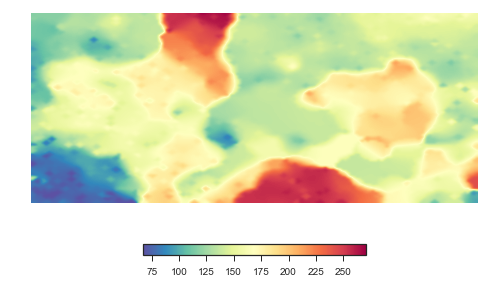
\includegraphics[width=.3\linewidth]{SOM/SOM_Prec8}}\hfill
	\subfloat[Prec9]{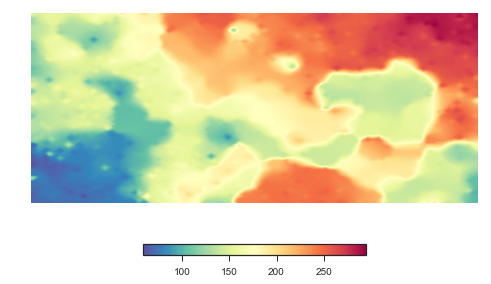
\includegraphics[width=.3\linewidth]{SOM/SOM_Prec9}}\hfill
	\newline
	\centering
	\subfloat[Prec10]{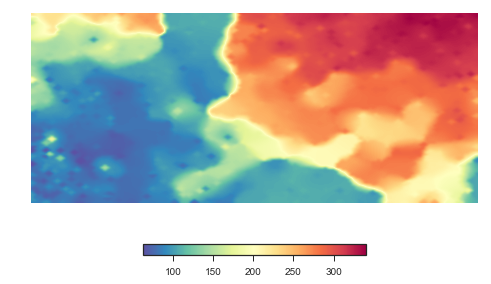
\includegraphics[width=.3\linewidth]{SOM/SOM_Prec10}}
	\subfloat[Average]{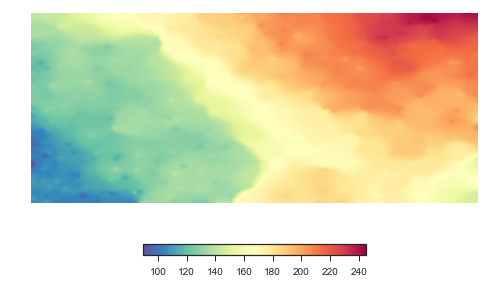
\includegraphics[width=.3\linewidth]{SOM/SOM_PrecTotalAvg}}
\end{figure}



\begin{figure}[H]
	\caption{SOM - Autres données}
	\centering
	\subfloat[Temp. Min. Average]{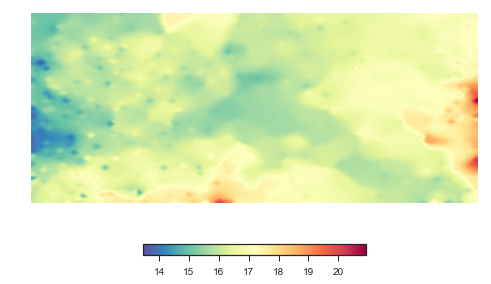
\includegraphics[width=.3\linewidth]{SOM/SOM_TminTotalAvg}}\hfill
	\subfloat[Temp. Max. Average]{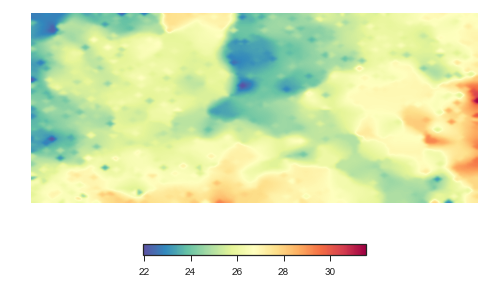
\includegraphics[width=.3\linewidth]{SOM/SOM_TmaxTotalAvg}}\hfill
	\subfloat[Temp. Mean. Average]{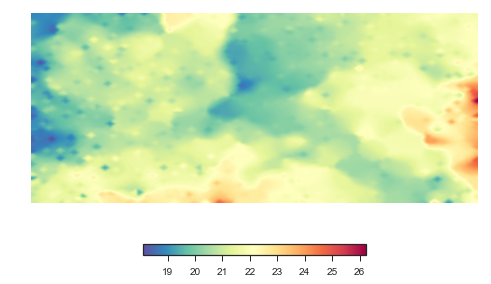
\includegraphics[width=.3\linewidth]{SOM/SOM_TmeanTotalAvg}}\hfill
	\newline
	\subfloat[Dtr Average]{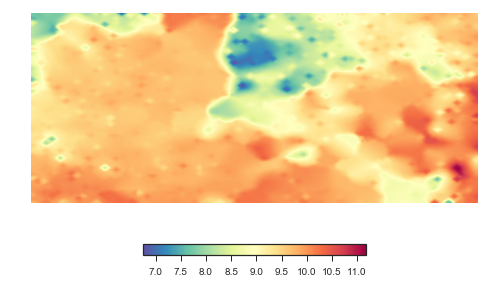
\includegraphics[width=.3\linewidth]{SOM/SOM_DtrTotalAvg}}\hfill
	\subfloat[ASNM]{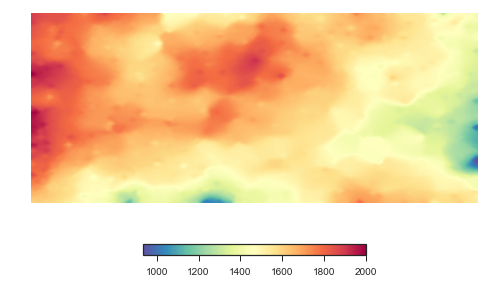
\includegraphics[width=.3\linewidth]{SOM/SOM_ASNM}}\hfill
	\subfloat[Slope]{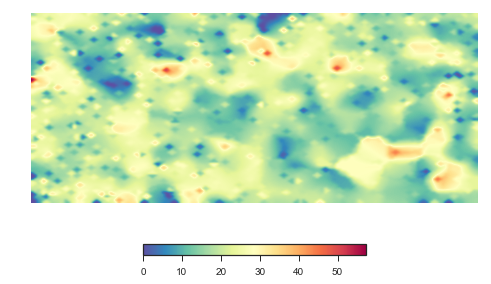
\includegraphics[width=.3\linewidth]{SOM/SOM_Slope}}\hfill
	\newline
	\subfloat[Franco]{\includegraphics[width=.3\linewidth]{SOM/SOM_Franco}}\hfill
	\subfloat[Arenoso]{\includegraphics[width=.3\linewidth]{SOM/SOM_Arenoso}}\hfill
	\subfloat[Arcilloso]{\includegraphics[width=.3\linewidth]{SOM/SOM_Arcilloso}}\hfill
	\newline
	\centering
	\subfloat[Limoso]{\includegraphics[width=.3\linewidth]{SOM/SOM_Limoso}}\hfill
	\subfloat[Cascajoso]{\includegraphics[width=.3\linewidth]{SOM/SOM_Cascajoso}}\hfill
	\subfloat[pH]{\includegraphics[width=.3\linewidth]{SOM/SOM_pHAvg}}\hfill
	\newline
	\subfloat[Organic]{\includegraphics[width=.3\linewidth]{SOM/SOM_OrgAvg}}\hfill
	\subfloat[Orientation]{\includegraphics[width=.3\linewidth]{SOM/SOM_OrientationDegrees}}\hfill
	\subfloat[Defectos]{\includegraphics[width=.3\linewidth]{SOM/SOM_DefectosTotales}}
\end{figure}



\begin{figure}[H]
	\caption{\label{SecondSOMASNM}Altitude et défauts lors d'une seconde exécution du réseau de neurones}
	\centering
	\subfloat[ASNM]{\includegraphics[width=.5\linewidth]{SOM/SOM_ASNM2}}\hfill
	\subfloat[Defectos Totales]{\includegraphics[width=.5\linewidth]{SOM/SOM_DefectosTotales2}}
	\newline

	\centering
	\subfloat[ASNM]{\includegraphics[width=.5\linewidth]{SOM/SOM_ASNM2}}\hfill
	\subfloat[Puntaje Total]{\includegraphics[width=.5\linewidth]{SOM/SOM_PuntajeTotal}}\hfill
	\newline
	\centering 
	\subfloat[Coffee Class Position]{\includegraphics[width=.5\linewidth]{SOM/SOM_Umatrix_Points_Category}}
\end{figure}


\noindent Afin de mieux visualiser la répartition des cafés d'année en année sur la carte SOM, une autre exécution a été réalisée\footnote{Les cartes SOM sont initialisées aléatoirement et les exécutions diffèrent les unes des autres. Il est difficile de sauvegarder l'environnement pour ensuite réaliser d'autres opérations sur les cartes.} et les années affichées. 


\begin{figure}[H]
	\caption{\label{ThirdSOMASNM}Répartition par année et mise en avant des composants intéressants de la SOM}
	\centering
	\subfloat[Umatrix]{\includegraphics[width=.5\linewidth]{SOM/SOM2/umatrix}}\hfill
	\subfloat[Defectos Totales]{\includegraphics[width=.5\linewidth]{SOM/SOM2/umatrix_defectos}}
	\newline
	
	\centering
	\subfloat[Precipitations]{\includegraphics[width=.5\linewidth]{SOM/SOM2/umatrix_prectotalavg}}\hfill
	\subfloat[Year, 2011 (Noir), 2016 (Orange)]{\includegraphics[width=.5\linewidth]{SOM/SOM2/umatrix_year}}\hfill
	\newline
	\centering 
	\subfloat[Coffee Class Position, same as \ref{umatrix_cat}]{\includegraphics[width=.5\linewidth]{SOM/SOM2/umatrix_cat}}
\end{figure}

\newpage
\paragraph{Analyse des cartes}On peut observer que les régions avec beaucoup de précipitations sont aussi celles qui ont le plus de cafés avec peu de points. Lors d'une seconde exécution du réseau on a pu observer une relation proche entre les défauts et l'altitude comme montré sur la figure \ref{SecondSOMASNM}. Cette relation n'était pas clairement visible lors de la première exécution. Le fait est déjà connu que le café qui pousse en altitude est de meilleure qualité cependant ici on remarque que les cafés cultivés aux altitudes les plus hautes sont les plus sujets à une grande quantité de défauts. Les défauts physiques n'interviennent que peu dans la qualité finale du café mais peuvent avoir une influence en cas de mauvais tri. On observe sur la figure \ref{AltPts} que la zone en bas à gauche, là où l'altitude est la plus haute, correspond à une zone possédant peu de cafés ayant eu le score 0 et beaucoup ayant eu des scores entre 85 et 90. Cependant, des cafés ayant un nombre de points de moins de 80 points, en rouge ou compris entre 89 et 85, en bleu, sont présents plus ou moins de manière homogène sur la totalité de la carte, indépendamment de l'altitude. Sur la figure \ref{ThirdSOMASNM} on peut observer que les fortes précipitations sont liées au nombre de défauts mais aussi fortement à l'année. Presque aucun des café de l'année 2011 n'a eu de score compris dans la catégorie 2. 


%TODO trouver le café à 90 points de 2011









\newpage

\section{Apprentissage supervisé}
%Il a été possible ou non de faire de la prédiction, confusion matrix etc
%ce que les méthodes comme random forest ont donné
Le but de cette section est d'analyser la possibilité de prédiction de la qualité des cafés\footnote{La qualité du café fait références aux variables dépendantes citées dans la section \ref{VarDep}.} à l'aide des données climatiques et de qualité de sols à disposition. Les méthodes Random Forest et Partial Least Squares seront utilisées.


\subsection{Random Forest}
 
Cette section présente comment la méthode Random Forest a été utilisée et les résultats produits. 
\subsubsection{Méthode utilisée}
% détails de la méthode, choix pour la cross validation, variables entrée/sortie 
Afin de se faire la meilleure idée possible des possibilités de prédiction, quatre variables de sorties ont été testées. Le nombre total de points (Puntaje Total), l'acidité (Acidez), la douceur (Dulzor) et la catégorie, obtenue d'après le tableau à la section \ref{categoriesCafe}. \\

\noindent La méthode Random Forest du package Caret a été utilisée avec une K-Fold Cross Validation ayant comme paramètre K = 10, répétée 3 fois. 

\begin{lstlisting}[caption={Fonction d'entrainement et de test du modèle avec Random Forest},captionpos=b]
	RFmodelCategory=train(x_cat,y_cat,method="rf",
	tunegrid=tunegrid_cat,
	trControl=trainControl(method="repeatedcv",number=10,repeats=3),
	tuneLength=10,importance = TRUE, proximity=T)
\end{lstlisting}




\newpage
\subsubsection{Résultats de classification}
% Nombre ,graphiques, analyses
En première partie, la tentative de classification avec comme variable de sortie la catégorie. Nous avons pour le modèle:

\begin{itemize}
	\item 490 échantillons \footnote{La totalité des échantillons ont été utilisés ici, y compris ceux possédant 0 points.}
	\item 72 variables indépendantes
	\item 3 classes ("2", "3", "4")
\end{itemize}

Re-échantillonnage des résultats parmi les paramètres de réglage:

\begin{table}[H]
	\centering
	\caption{Réglage du modèle}
	\label{RF_Class_Resampling}
	\begin{tabular}{lll}
		mtry & Accuracy  & Kappa      \\
		2    & 0.4995912 & 0.08462730 \\
		9    & 0.5117305 & 0.10653423 \\
		17   & 0.5062583 & 0.09657805 \\
		25   & 0.5109109 & 0.10608506 \\
		33   & 0.5075520 & 0.10148125 \\
		40   & 0.5014028 & 0.08705477 \\
		48   & 0.5088592 & 0.10056043 \\
		56   & 0.5095934 & 0.10397803 \\
		64   & 0.5081794 & 0.10110968 \\
		72   & 0.5061636 & 0.09829896           
	\end{tabular}
\end{table}

\noindent On observe qu'avec un \textit{mtry}\footnote{À chaque split de l'arbre, l'algorithme va chercher \textit{mtry} variables dans le set. Chaque nouveau split sera composté de \textit{mtry} variables sélectionnées aléatoirement dans le set de donnée principal} de 9, l'\textit{Accuracy} est la meilleure .


\begin{table}[H]
	\centering
	\caption{Les vingt variables les plus importantes par catégorie (sur 72) pour la classification}
	\label{RF_Class_Impvar}
	\begin{tabular}{llll}
		& 2      & 3      & 4      \\
		ASNM      & 60.754 & 38.042 & 100.00 \\
		prec9     & 64.442 & 8.963  & 90.27  \\
		tmin5     & 1.302  & 30.008 & 87.63  \\
		dtr7      & 86.974 & 69.378 & 54.59  \\
		tmean1    & 12.041 & 42.173 & 86.82  \\
		prec10    & 29.188 & 30.604 & 82.33  \\
		tmin4     & 16.840 & 56.842 & 79.80  \\
		tmax5     & 8.655  & 51.687 & 76.56  \\
		tmin1     & 21.357 & 56.763 & 75.76  \\
		tmax4     & 29.270 & 71.631 & 26.10  \\
		tmean2    & 12.710 & 42.159 & 71.51  \\
		tmean5    & 18.301 & 37.089 & 70.87  \\
		dtr5      & 16.198 & 70.822 & 39.11  \\
		tmax8     & 9.814  & 50.375 & 70.72  \\
		dtr8      & 10.785 & 43.304 & 70.20  \\
		tmax6     & 18.386 & 68.704 & 51.16  \\
		prec6     & 40.057 & 25.298 & 68.17  \\
		DtrTotal  & 13.864 & 67.471 & 36.17  \\
		Cascajoso & 42.708 & 54.120 & 65.70  \\
		tmax10    & 6.866  & 45.774 & 65.59  \\
		&        &        &        \\
		&        &        &       
	\end{tabular}
\end{table}

\noindent Enfin après avoir construit le modèle, on peut le valider avec nos données de test. Nous obtenons les résultats suivants: 


\begin{figure}[H]
	\centering
	\includegraphics[scale=0.4]{../../Bachelor_Thesis_2017_Sources/Notebook/R/Projects/BachelorThesis/RF_models_perfs/ConfusionMatrix_RF_Classification_Result}
	\caption{Matrice de confusion de la classification avec Random Forest}
	\label{fig:confusionmatrixrfclassificationresult}
\end{figure}

\begin{minipage}{\linewidth}
	
	\begin{lstlisting}[showstringspaces=false,language=R, caption={Test du modèle de classification},captionpos=b]
		
		          Reference
	Prediction  2  3  4
		2   2  1  2
		3   9 50 50
		4   3 43 47
		
		
		Overall Statistics
		
		Accuracy : 0.4783          
		95% CI : (0.4085, 0.5486)
		No Information Rate : 0.4783          
		P-Value [Acc > NIR] : 0.52732         
		
		Kappa : 0.0416          
		Mcnemar's Test P-Value : 0.06796         
		
 Statistics by Class:
		
                      Class: 2 Class: 3 Class: 4
Sensitivity          0.142857   0.5319   0.4747
Specificity          0.984456   0.4779   0.5741
Pos Pred Value       0.400000   0.4587   0.5054
Neg Pred Value       0.940594   0.5510   0.5439
Prevalence           0.067633   0.4541   0.4783
Detection Rate       0.009662   0.2415   0.2271
Detection Prevalence 0.024155   0.5266   0.4493
Balanced Accuracy    0.563657   0.5049   0.5244
	\end{lstlisting}
\end{minipage}





%-------------------------------------------------------------------------

\newpage
\subsubsection{Régression sur la variable dépendante \textit{Puntaje Total}}
\noindent Notre modèle contient: 
\begin{itemize}
	\item 448 échantillons
	\item 72 variables indépendantes
\end{itemize}


\begin{table}[H]
	\centering
	\caption{Réglage du modèle}
	\label{RF_Total_Resampling}
	\begin{tabular}{llll}
		mtry & RMSE     & Rsquared     \\
		2    & 6.033466 & 0.03056280   \\
		9    & 6.063304 & 0.03686526   \\
		17   & 6.042679 & 0.04446260   \\
		25   & 6.056445 & 0.04747083   \\
		33   & 6.064986 & 0.05062423   \\
		40   & 6.052046 & 0.05279225   \\
		48   & 6.076724 & 0.05268180   \\
		56   & 6.084703 & 0.05124400   \\
		64   & 6.066546 & 0.05294682   \\
		72   & 6.079099 & 0.05567081    
	\end{tabular}
\end{table}

\noindent On observe qu'avec un \textit{mtry} de 2, la RMSE est la plus petite. Cependant, une fois testé le modèle donne l'erreur suivante: RMSE = 7.1726 et Rsquared = 0.00431. 


\begin{figure}[H]
	\centering
	\includegraphics[width=0.9\linewidth]{../../Bachelor_Thesis_2017_Sources/Notebook/R/Projects/BachelorThesis/RF_models_perfs/modele_Total_Regression}
	\caption{Performances de la régression pour la variable \textit{Puntaje Total}}
	\label{fig:modeletotalregression}
\end{figure}

\begin{minipage}{\linewidth}
	
	\begin{lstlisting}[showstringspaces=false,language=R, caption={Test du modèle de classification},captionpos=b]
	Call:
	randomForest(x = x, y = y, mtry = param$mtry, 
	importance = TRUE,
	proximity = ..3, tunegrid = ..1) 
	
	Type of random forest: regression
	Number of trees: 500
	No. of variables tried at each split: 2
	
	Mean of squared residuals: 38.38491
	% Var explained: -9.59
	
	\end{lstlisting}
\end{minipage}


\begin{table}[H]
	\centering
	\caption{Les 20 variables les plus importantes du modèle.}
	\label{RF_Total_Varimp}
	\begin{tabular}{ll}
		& Overall \\
		tmean2       & 100.00  \\
		tmax6        & 99.28   \\
		tmean4       & 96.71   \\
		tmax2        & 94.71   \\
		tmax5        & 92.77   \\
		PrecTotalAvg & 90.81   \\
		tmax4        & 88.96   \\
		dtr4         & 88.89   \\
		tmin2        & 87.82   \\
		DtrTotal     & 87.43   \\
		tmin3        & 87.25   \\
		tmin5        & 86.97   \\
		tmean1       & 86.93   \\
		tmean8       & 85.72   \\
		tmax8        & 85.34   \\
		TminTotalAvg & 84.71   \\
		dtr2         & 84.71   \\
		tmean10      & 84.42   \\
		tmin1        & 83.93   \\
		prec10       & 83.85  
	\end{tabular}
\end{table}



\begin{figure}[H]
	\centering
	\includegraphics[width=0.7\linewidth]{../../Bachelor_Thesis_2017_Sources/Notebook/R/Projects/BachelorThesis/RF_models_perfs/Pred_PuntajeTotal}
	\caption{Comparaison des prédiction et des valeurs actuelle pour la variable \textit{Puntaje Total}}
	\label{fig:predpuntajetotal}
\end{figure}



%-----------------------------------------------------------------------


\newpage
\subsubsection{Régression sur la variable dépendante \textit{Acidez}}
\noindent Notre modèle contient: 
\begin{itemize}
	\item 448 échantillons
	\item 72 variables indépendantes
\end{itemize}


\begin{table}[H]
	\centering
	\caption{Réglage du modèle}
	\label{RF_Acidez_Resampling}
	\begin{tabular}{llll}
	    mtry & RMSE      & Rsquared   \\
	    2    & 0.5523984 & 0.07780696 \\
	    9    & 0.5587745 & 0.07205180 \\
	    17   & 0.5591882 & 0.07332069 \\
	    25   & 0.5614777 & 0.07128568 \\
	    33   & 0.5601199 & 0.07188263 \\
	    40   & 0.5602361 & 0.07391410 \\
	    48   & 0.5608331 & 0.07075389 \\
	    56   & 0.5599010 & 0.07333161 \\
	    64   & 0.5604395 & 0.07236162 \\
	    72   & 0.5607297 & 0.07082403
	\end{tabular}
\end{table}

\noindent On observe qu'avec un \textit{mtry} de , la RMSE est la plus petite. Cependant, une fois entrainé le modèle donne l'erreur suivante: RMSE = 0.5587  et Rsquared = 0.0261. 

\begin{figure}[H]
	\centering
	\includegraphics[width=0.9\linewidth]{../../Bachelor_Thesis_2017_Sources/Notebook/R/Projects/BachelorThesis/RF_models_perfs/modele_Acidez_regression}
	\caption{Performances de la régression pour la variable \textit{Acidez}}
	\label{fig:modeleacidezregression}
\end{figure}


\begin{minipage}{\linewidth}
	
	\begin{lstlisting}[showstringspaces=false,language=R, caption={Test du modèle de classification},captionpos=b]
	Call:
	randomForest(x = x, y = y, mtry = param$mtry, 
	importance = TRUE,      
	proximity = ..3, tunegrid = ..1) 
	Type of random forest: regression
	Number of trees: 500
	No. of variables tried at each split: 2
	
	Mean of squared residuals: 0.3157974
	% Var explained: -1.63
	\end{lstlisting}
\end{minipage}


\begin{table}[H]
	\centering
	\caption{Les 20 variables les plus importantes du modèle.}
	\label{RF_Acidez_Varimp}
	\begin{tabular}{ll}
	 & Overall \\
	 dtr10         & 100.00  \\
	 tmin9         & 98.16   \\
	 tmean3        & 96.84   \\
	 tmax8         & 96.40   \\
	 tmax7         & 94.54   \\
	 tmax6         & 93.25   \\
	 tmin3         & 92.78   \\
	 TmeanTotalAvg & 90.41   \\
	 DtrTotalAvg   & 89.54   \\
	 tmax3         & 89.17   \\
	 TmaxTotalAvg  & 88.40   \\
	 tmax5         & 87.07   \\
	 tmax10        & 85.38   \\
	 TminTotalAvg  & 84.12   \\
	 dtr8          & 83.90   \\
	 tmean10       & 83.73   \\
	 tmin5         & 83.27   \\
	 tmax1         & 82.81   \\
	 tmean4        & 82.49   \\
	 tmean9        & 81.66  
	\end{tabular}
\end{table}

\begin{figure}[H]
	\centering
	\includegraphics[width=0.7\linewidth]{../../Bachelor_Thesis_2017_Sources/Notebook/R/Projects/BachelorThesis/RF_models_perfs/Pred_ACidez}
	\caption{Comparaison des prédiction et des valeurs actuelle pour la variable \textit{Acidez}}
	\label{fig:predacidez}
\end{figure}


%TODO plot acidez vs altitude ou pas
%LA RMSE est bonne ici -> regarder Rsquared, car pas dépendent de l'unité, si proche de 1 c'est bon sinon c'est dela merde ->  c'est toujours de la merde -> commentj'aie u peur d'un coup !


%-----------------------------------------------------------------------


\newpage
\subsubsection{Régression sur la variable dépendante \textit{Dulzor}}
\noindent Notre modèle contient: 
\begin{itemize}
	\item 439 échantillons
	\item 72 variables indépendantes
\end{itemize}


\begin{table}[H]
	\centering
	\caption{Réglage du modèle}
	\label{RF_Dulzor_Resampling}
	\begin{tabular}{llll}
	mtry & RMSE      & Rsquared   \\
	2    & 0.7996682 & 0.02423378 \\
	9    & 0.8030381 & 0.03690104 \\
	17   & 0.8082138 & 0.04453890 \\
	25   & 0.8112174 & 0.04482055 \\
	33   & 0.8141780 & 0.04452465 \\
	40   & 0.8163036 & 0.04853452 \\
	48   & 0.8187376 & 0.04858482 \\
	56   & 0.8211659 & 0.04628629 \\
	64   & 0.8209675 & 0.04722086 \\
	72   & 0.8226232 & 0.04976240
	\end{tabular}
\end{table}

\noindent On observe qu'avec un \textit{mtry} de 2, la RMSE est la plus petite. Cependant, une fois entrainé le modèle donne l'erreur suivante: RMSE = 0.8747  et Rsquared = 0.0009. 

\begin{figure}[H]
	\centering
	\includegraphics[width=0.9\linewidth]{../../Bachelor_Thesis_2017_Sources/Notebook/R/Projects/BachelorThesis/RF_models_perfs/modele_dulzor_regression}
	\caption{Performances de la régression pour la variable \textit{Dulzor}}
	\label{fig:modeledulzorregression}
\end{figure}



\begin{minipage}{\linewidth}
	
	\begin{lstlisting}[showstringspaces=false,language=R, caption={Test du modèle de classification},captionpos=b]
Call:
randomForest(x = x, y = y, mtry = param$mtry, 
importance = TRUE,      
proximity = ..3, tunegrid = ..1) 
Type of random forest: regression
Number of trees: 500
No. of variables tried at each split: 2

Mean of squared residuals: 0.7230219
% Var explained: -9.25
	\end{lstlisting}
\end{minipage}


\begin{table}[H]
	\centering
	\caption{Les 20 variables les plus importantes du modèle.}
	\label{RF_Dulzor_Varimp}
	\begin{tabular}{ll}
              & Overall \\
dtr4          & 100.00  \\
tmax4         & 99.29   \\
tmax9         & 96.55   \\
tmin4         & 93.13   \\
tmean4        & 92.17   \\
TmaxTotal     & 91.49   \\
tmin5         & 90.85   \\
TmeanTotal    & 90.64   \\
prec6         & 89.90   \\
tmin2         & 89.84   \\
dtr10         & 89.69   \\
tmax6         & 89.17   \\
tmax5         & 87.47   \\
tmax7         & 87.16   \\
dtr8          & 87.15   \\
tmax2         & 86.37   \\
dtr2          & 86.23   \\
tmean1        & 85.78   \\
TmeanTotalAvg & 85.08   \\
DtrTotal      & 84.98
	\end{tabular}
\end{table}


\begin{figure}[H]
	\centering
	\includegraphics[width=0.7\linewidth]{../../Bachelor_Thesis_2017_Sources/Notebook/R/Projects/BachelorThesis/RF_models_perfs/Pred_Dulzor}
	\caption{Comparaison des prédiction et des valeurs actuelle pour la variable \textit{Dulzor}}
	\label{fig:preddulzor}
\end{figure}


\newpage


%TODO Footnote pour kappa
\paragraph{Discussion des résultats pour Random Forest}
Avec une \textit{accuracy} de seulement 0.47  (47\% d'échantillons classés correctement) et un test de Kappa d'uniquement 0.0416, la classification à l'aide de Random Forest ne semble pas fiable avec les données en notre possession. \\

\noindent Pour mesurer la qualité de la régression, nous utiliserons comme mesure le coefficient $r^2$ fournit par les résultats de Random Forest. Plus le coefficient s'approche de $1$ plus la variation totale des sorties prédites par le modèle est faible et donc plus le modèle est bon. Les résultats obtenus avec les 3 variables de sortie différentes sont les suivants: \\


\begin{itemize}
	\item Puntaje Total: $r^2 = 0.00431$
	\item Acidez: $r^2 = 0.0261$
	\item Dulzor: $r^2 = 0.0009$
\end{itemize} 












%TODO finir RF et parler de RF avec les variables sans variance etc
\subsection{Random Forest avec variables à haute variabilité}
Afin de tester le modèle sans données inutilement redondantes et fortement corrélées, un second modèle Random Forest a été entrainé avec les variables indépendantes qui avaient un taux de variabilité supérieur à un certain niveau. Le premier niveau a été placé à $10$, ce qui a pour effet de ne garder que $25$ variables. Le second a été placé à $20$, ce qui a pour effet de ne garder que $21$ variables. Les résultats se sont avérés tout aussi imprécis, voir par exemple les résultats de prédiction sur la figure \ref{fig:rfptotalvariability10} avec le seuil à 10 pour la variable \textit{Puntaje Total} et sur la figure \ref{fig:rfptotalvariability20} avec le seuil à 20. Les cafés ayant un total de zéro points ont ici été gardés afin d'observer une éventuelle prédiction correspondante. Sur la figure \ref{fig:rfptotalvariability10} on peut observer qu'un des café ayant zéro points a été prédit à moins de 40 points. Les variables montrée dans le tableau \ref{tab:variability10Variables} sont celles utilisées pour créer le modèle avec un seuil de 10. On peut voir que les précipitations ont une grande importance et cela rejoint l'idée observée dans la section \ref{SOM} que la quantité de précipitations est importante pour la qualité du grain, cependant cela ne permet que d'avoir une approximation de la quantité de défauts physique du grain et non sur la qualité générale. 

\begin{figure}[H]
	\centering
	\includegraphics[width=0.7\linewidth]{../../Bachelor_Thesis_2017_Sources/Notebook/R/Projects/BachelorThesis/RF_models_perfs/RF_PTotal_Variability10}
	\caption{Prédiction du total de points avec 25 variables indépendantes}
	\label{fig:rfptotalvariability10}
\end{figure}
\begin{figure}[H]
	\centering
	\includegraphics[width=0.7\linewidth]{../../Bachelor_Thesis_2017_Sources/Notebook/R/Projects/BachelorThesis/RF_models_perfs/RF_PTotal_Variability20}
	\caption{Prédiction du total de points avec 21 variables indépendantes}
	\label{fig:rfptotalvariability20}
\end{figure}





\begin{table}[H]
	\centering
	\caption{Variables à haute variabilité avec un coefficient de variabilité supérieur à 10}
	\label{tab:variability10Variables}
	\begin{tabular}{lll}
		& \%IncMSE   & IncNodePurity \\
		ASNM           & 5.0408727  & 15044.3045    \\
		Luminosidad    & 5.4787179  & 3642.4806     \\
		prec1          & 7.6033403  & 11395.8391    \\
		prec2          & 8.4894841  & 12991.3588    \\
		prec3          & 9.6477012  & 14018.6199    \\
		prec4          & 7.6742913  & 16432.9873    \\
		prec5          & 8.5170477  & 13554.8590    \\
		prec6          & 9.3037427  & 14994.6836    \\
		prec7          & 7.3229410  & 14325.6941    \\
		prec8          & 9.0394682  & 13509.3978    \\
		prec9          & 9.6867243  & 13287.9725    \\
		prec10         & 12.0962566 & 17472.3424    \\
		dtr5           & 10.2926692 & 16738.1273    \\
		dtr10          & 9.1992584  & 15261.9880    \\
		PrecTotal      & 12.0991208 & 15483.9130    \\
		PrecTotalAvg   & 11.6456487 & 13780.0364    \\
		OrientationNum & 2.4731816  & 10925.6272    \\
		Slope          & 0.1353807  & 15492.9382    \\
		org\_avg       & 2.7056077  & 6520.6197     \\
		Franco         & 1.5936970  & 1931.0307     \\
		Arcilloso      & -2.9621275 & 1746.0451     \\
		Limoso         & 2.7839655  & 1631.1038     \\
		Arenoso        & -1.5199547 & 831.4292      \\
		Cascajoso      & -0.5423810 & 2330.3915    
	\end{tabular}
\end{table}














\newpage

\subsection{Partial Least Squares}
% analyser les résultats de prédiction ainsi que les corrélation fournies par PLS - au vus des résultats et de la corrélation entre les variables de sorties pas besoind 'utiliser MBPLS ça serait une perte de temps
Cette méthode utilise à la fois le principe de régression et d'analyse en composante principale (PCA ou ACP). La méthode \textit{plsreg1} de R fournit en retour plusieurs objets dont les corrélation entre variable dont la représentation graphique permet de visualiser aisément où se placent les variables de sorties choisie. 

\begin{figure}[H]
	\centering
	\includegraphics[scale=0.5]{../../Bachelor_Thesis_2017_Sources/Notebook/R/Projects/BachelorThesis/PLS/CircleOfCorrelationPuntajeTotal}
	\caption{Représentation des corrélations entre les variables indépendantes et la variable dépendante \textit{Puntaje Total}}
	\label{fig:circleofcorrelationpuntajetotal}
\end{figure}
 
\begin{figure}[H]
	\centering
	\includegraphics[scale=0.5]{../../Bachelor_Thesis_2017_Sources/Notebook/R/Projects/BachelorThesis/PLS/CircleOfCorrelationAcidez}
	\caption{Représentation des corrélations entre les variables indépendantes et la variable dépendante \textit{Acidez}}
	\label{fig:circleofcorrelationacidez}
\end{figure}

\begin{figure}[H]
	\centering
	\includegraphics[scale=0.5]{../../Bachelor_Thesis_2017_Sources/Notebook/R/Projects/BachelorThesis/PLS/CircleOfCorrelationDulzor}
	\caption{Représentation des corrélations entre les variables indépendantes et la variable dépendante \textit{Dulzor}}
	\label{fig:circleofcorrelationdulzor}
\end{figure}


\subsubsection{Analyse des résultats}

La prédiction avec Partial Least Squares ne donne pas de résultats plus convainquant que Random Forest. Cependant et afin de mitiger ces résultats, la méthode n'a pas été exploitée avec son plein potentiel car un seul block de donnée à été utilisé (la totalité des variables indépendantes) alors que PLS et Multiblock PLS peuvent éventuellement être amélioré en réglant les paramètres plus finement. 

\begin{figure}[H]
	\centering
	\includegraphics[width=0.7\linewidth]{../../Bachelor_Thesis_2017_Sources/Notebook/R/Projects/BachelorThesis/PLS/ComparisonOfResponsesPuntajeTotal}
	\caption{Comparaison des prédiction et des valeurs actuelle pour la variable Puntaje Total}
	\label{fig:comparisonofresponsespuntajetotal}
\end{figure}


\begin{figure}[H]
	\centering
	\includegraphics[width=0.7\linewidth]{../../Bachelor_Thesis_2017_Sources/Notebook/R/Projects/BachelorThesis/PLS/ComparisonOfResponsesAcidez}
	\caption{Comparaison des prédiction et des valeurs actuelle pour la variable Acidez}
	\label{fig:comparisonofresponsesacidez}
\end{figure}



\begin{figure}[H]
	\centering
	\includegraphics[width=0.7\linewidth]{../../Bachelor_Thesis_2017_Sources/Notebook/R/Projects/BachelorThesis/PLS/ComparisonOfResponsesDulzor}
	\caption{Comparaison des prédiction et des valeurs actuelle pour la variable Dulzor}
	\label{fig:comparisonofresponsesdulzor}
\end{figure}




















	
	\chapter{Discussion des résultats}


%Analyse globale des résultats, discussion sur les résultats 
%Données manquantes

%Exemple: on sait que la fermentation du grain dans sa pulpe impacte sur la chimie de la graine et peut rendre le café plus ou moins acide -> pas de données sur la fermentation (temps, méthode etc) idem pour le séchage, le stockage, la récolte etc


% L'objectif aurait été de définir des gouts (tastewheel ) - pas de données

% Revenir sur les données 

% todo -> améliorer les modèles, changer les index (RMSE, RSquared etc) - nécessite théorie

% Portes qui s'ouvrent 

%TODO - Relire et relire, revenir surle rapport et relire, penser au résumé etc

Les différentes analyses réalisées, tant au niveau de l'apprentissage supervisé que non-supervisé n'ont pas permis de créer un modèle fiable de description ou de prédiction de la qualité du café. Cependant, certains résultats peuvent être mis en avant et certaines critiques peuvent être faites sur les données et les méthodes utilisées. \\

%Relation avec la pluie
\paragraph{Résultats exploitables} Concernant les résultats exploitables, une relation a été observée entre la quantité de pluie durant l'année et le nombre de défauts physiques du grain. Plus il y a de pluie, plus il y a de grains ayant des défauts et plus il y a de cafés ayant la note zéro (voir figure \ref{ThirdSOMASNM}). Rappelons que les grains défectueux sont éliminés par un processus industriel permettant l'élimination des grains ayant une couleur ou une densité anormale. Cependant, certains défauts, comme la présence de trous dûs aux parasites (Broca, ou Broca de punto), sont plus difficilement détectables et peuvent amener un goût désagréable au café. Un seul grain peut modifier le goût d'une tasse ! On remarque aussi que l'année 2011 a beaucoup moins de cafés dont la note dépasse les 80 (voir figure \ref{fig:pointtotauxetc}), score minimal pour avoir ma mention \textit{Specialty Coffee}. Il est donc raisonnable de penser que les fortes quantités de pluie, nuisent à la qualité du café et que plus il pleut, moins il y a de chance d'avoir de très bon cafés.  \\



% Manque de données
\paragraph{Données disponibles} Certain points concernant la qualité des données reçues sont à mettre en avant. Premièrement, les données de qualités de sols ne contenant que le pH, le taux de matières organiques et la texture, toutes les relations chimiques éventuelles entre les minéraux du sol et les arômes n'ont pas pu être explorées. La composition chimique du sol n'est pas la seule à avoir une influence possible sur la qualité et les saveurs du café. Les différents traitement du café une fois récolté, comme la fermentation ou le séchage, peuvent avoir une grande influence mais malheureusement aucune donnée n'a été fournie à ce sujet non plus. \\

\noindent Deuxièmement, les données de dégustation contenaient parfois, de manière difforme, des notes sur les arômes ou saveurs du café. Ces données peuvent être décrites comme sur la figure \ref{fig:coffeeflavorwheel} et pourraient permettre de décrire d'une manière plus sensorielle le goût du café et ainsi faire un éventuel lien avec les composants chimiques du sol et les pratiques culturales ou même le climat. Malheureusement, le manque de données en nombre d'une part et d'uniformité d'autre part n'ont pas permis d'intégrer ces informations au set de données et donc d'en analyser les éventuelles corrélations.\\

\begin{figure}[h]
	\centering
	\includegraphics[width=1\linewidth]{img/coffee_flavor_wheel}
	\caption{Roue des parfums du café}
	\label{fig:coffeeflavorwheel}
\end{figure}



%Customisation des méthodes, essais avec d'autres méthodes, traitement des variables catégorielles

%parler des données d'Eric sur la plante du café, de la taille etc



\noindent Il serait intéressant de prélever d'autres données, directement au niveau des fermes. Beaucoup de facteurs influencent la croissance d'une plante et la maturation de ses fruits en particulier les facteurs influençant la photosynthèse. Si une plante est particulièrement exposée à l'est, et donc au soleil du matin, la photosynthèse sera plus efficace car l'humidité ambiante est plus élevée, ce qui améliore les capacités d'assimilation de la lumière par la plante. Par contre, si la plante grandit sur un terrain ombragé, donc entourée d'autres plantes, l'humidité sera aussi plus élevée mais la plante devra fabriquer plus de feuilles pour capter plus de lumière et aura donc moins d'énergie à mettre dans les fruits. L'altitude peut aussi avoir une influence importante. Sur la luminosité, en particulier par rapport à la couverture nuageuse qui peut être parfois plus importante en montagne, mais aussi sur la température. Dans les lieux plus froids, la plante fonctionne plus lentement et les fruits ont besoin de plus de temps pour murir, ce qui laisse plus de temps aux arômes pour se développer et produit de manière générale des cafés de qualités.  \\



% si on veut prédire la qualité du café, il faut des données précises. Il peut pleuvoir des trombes sur une ferme, et 100m plus loin rien. 



%Résultat
\noindent Durant le projet, une réunion a été organisée avec Felipe Rincón, coordonnateur de gestion au comité départemental des caféiculteurs de Risaralda, qui est à l'origine des données sur le café que nous avons reçues. La possibilité m'a été donnée de poser des questions entre autre sur le processus de récolte et de centralisation des données, processus jusqu'alors inexistant. M. Rincón m'a alors confié que les différentes demandes effectuées pour ce travail ainsi que le résultat final de l'agglomération des données disponibles, l'ont poussé à commencer un processus de normalisation de la récolte des données. Il est donc envisageable de pouvoir retenter une étude de ce type lorsque les données existantes auront éventuellement été complétées et lorsque de nouvelles données, plus complètes et possédant moins de défauts, auront été générées. Parmi les défauts importants signalés à M. Rincón, on notera qu'aucune date de récolte n'a été fournie. Seul les dates de dégustation étaient disponibles et les périodes de croissance de la plante ont dû être estimées. \\


\paragraph{Méthodes utilisées} Il est aussi important de mentionner les méthodes utilisées. Random Forest, PLS, ou le clustering, peuvent être paramétrées de beaucoup de manières différentes et leur efficacité peut être testée et améliorée. Dans le cadre de ce projet, avec le peu d'heures à disposition, ces méthodes ont été utilisées de manière exploratoire afin d'avoir une première impression sur les possibilités de modélisation. D'un même point de vue, d'autres méthodes auraient pu être explorées en jouant sur les particularités de chacune d'entre-elles par rapport aux types de données en notre possession. Pour améliorer cette partie, un bagage théorique supplémentaire en statistique serait nécessaire afin de mieux cerner les subtilités des méthodes de modélisation.  \\

\noindent 


 














	
	

\chapter{Conclusion}
Qu'est-ce que le travail peut apporter, que faudrait-il faire pour qu'il apporte plus (données manquantes, autres méthodes à explorer) 


	
	\backmatter
	
	\appendix

\chapter{Description des données}
\section{Dataset}
Le dataset présenté ci-dessous a été réalisé en regroupant les informations de plusieurs classeurs Excel ainsi que de documents au format PDF. Il s'agit d'une version contenant la totalité des données nécessaire au pré-traitement comme les coordonnées géographiques, les noms des fermes etc. Des sous-sets ont été extraits selon les besoins afin de réaliser les calculs avec, par exemple, uniquement les valeurs numériques et une variable dépendante spécifique. 



\begin{table}[H]
	\centering
	\caption{Dataset partie 1}
	\label{my-label}
	\begin{tabular}{ll}
		SICA            & Numéro d'identification unique par parcelle        \\
		Cedula          & Numéro de document d'identité du caféiculteur      \\
		Municipio       & Municipio                                          \\
		Vereda          & Vereda                                             \\
		Finca           & Ferme                                              \\
		EPSG:3116\_X    & Coordonnées                                        \\
		EPSG:3116\_Y    & Coordonnées                                        \\
		EPSG:4326\_Y    & Coordonnées                                        \\
		EPSG:4326\_X    & Coordonnées                                        \\
		Variedad        & Variété                                            \\
		FechaAnalysis   & Date d'analyse                                     \\
		year            & Année d'analyse                                    \\
		Occurence       & Nombre d'occurrence du café                        \\
		UV              & Pas d'information                                  \\
		Olor            & Pas d'information                                  \\
		Humedad         & Humidité                                           \\
		Merma           & Ullage                                             \\
		Pergamino       & Produit après lavage                               \\
		Almendra        & Uniformité des grains                              \\
		AlmendraTotal   & Total de grain                                     \\
		AlmendraSana    & Total de grain sains                               \\
		NegrosYVinagres & Défaut physique                                    \\
		Broca           & Défaut physique                                    \\
		\end{tabular}
\end{table}
\begin{table}[H]
\centering
\caption{Dataset partie 2}
\label{my-label}
\begin{tabular}{ll}
		BrocaDePunto    & Défaut physique                                    \\
		Veteado         & Défaut physique                                    \\
		Mordido         & Défaut physique                                    \\
		Inmaduro        & Défaut physique                                    \\
		Flojo           & Défaut physique                                    \\
		Sobresecado     & Défaut physique                                    \\
		Arrugado        & Défaut physique                                    \\
		Aplastado       & Défaut physique                                    \\
		Cristalizado    & Défaut physique                                    \\
		Reposado        & Défaut physique                                    \\
		Granizo         & Défaut physique                                    \\
		Conchas         & Défaut physique                                    \\
		Partido         & Défaut physique                                    \\
		Ambar           & Défaut physique                                    \\
		DefectosTotales & Total des défauts                                  \\
		ASNM            & Altitude  {[}mètres{]}                             \\
		Luminosidad     & Luminosité (3 catégories)                          \\
		prec1-10        & Précipitations sur 10 mois                         \\
		tmin1-10        & Températures min sur 10 mois                       \\
		tmax1-10        & Températures max sur 10 mois                       \\
		tmean1-10       & Températures moyennes sur 10 mois                  \\
		dtr1-10         & Diurnal Temperature Range sur 10 mois              \\
		PrecTotal       & Total des précipitations                           \\
		TminTotal       & Total des températures minimales                   \\
		TmaxTotal       & Total des températures maximales                   \\
		TmeanTotal      & Total des températures moyennes                    \\
		DtrTotal        & Total des DTR                                      \\
		PrecTotalAvg    & Moyenne des prec sur 10 mois                       \\
		TminTotalAvg    & Moyenne des tmin sur 10 mois                       \\
		TmaxTotalAvg    & Moyenne des tmax sur 10 mois                       \\
		TmeanTotalAvg   & Moyenne des tmean sur 10 mois                      \\
		DtrTotalAvg     & Moyenne des DTR sur 10 mois                        \\
		OrientationNum  & Orientation N-S-E-W {[}8 catégories{]}             \\
		Slope           & Pente {[}pourcentage{]}                            \\
		Soil Profile    & Profil du sol                                      \\
		Unidad\_c\_1    & Sous-profil                                        \\
		pH\_avg         & pH moyen sur 1m                                    \\
	\end{tabular}
\end{table}
\begin{table}[H]
\centering
\caption{Dataset partie 3}
\label{my-label}
\begin{tabular}{ll}
		org\_avg        & Matière organique moyenne sur 1m {[}pourcentage{]} \\
		Franco          & Sol Franco {[}0,1,2,3{]}                           \\
		Arcilloso       & Sol Argilleux {[}0,1,2,3{]}                        \\
		Limoso          & Sol Limoneux {[}0,1,2,3{]}                         \\
		Arenoso         & Sol Sabloneux {[}0,1,2,3{]}                        \\
		Cascajoso       & Sol Gravilloneux {[}0,1,2,3{]}                     \\
		Taza1           & Tasse une (limpia ou non)                          \\
		Taza2           & Tasse deux (limpia ou non)                         \\
		Taza3           & Tasse trois (limpia ou non)                        \\
		Taza4           & Tasse quatre (limpia ou non)                       \\
		Taza5           & Tasse cinq (limpia ou non)                         \\
		Aroma-Fragancia & Parfum-Arome {[}0-10 pts{]}                        \\
		Acidez          & Acidité {[}0-10 pts{]}                             \\
		Cuerpo          & Corps {[}0-10 pts{]}                               \\
		Sabor           & Saveur {[}0-10 pts{]}                              \\
		SaborResidual   & Saveur résiduelle {[}0-10 pts{]}                   \\
		Dulzor          & Douceur  {[}0-10 pts{]}                            \\
		Uniformidad     & Uniformité {[}0-10 pts{]}                          \\
		Balance         & Equilibre {[}0-10 pts{]}                           \\
		TazaLimpia      & Tasse "propre" {[}0-10 pts{]}                      \\
		PuntajeCatador  & Points dégustateur {[}0-10 pts{]}                  \\
		PuntajeTotal    & Points totaux {[}0-100 pts{]}                      \\
		Category        & Catégorie {[}1,2,3,4{]}                           
	\end{tabular}
\end{table}
 

\section{Données de dégustation brutes}
Les nombreux fichiers sont disponibles dans les sources du projet. 

\section{Données climatiques et géographiques brutes}
Les données climatiques consistent en l'extrapolation de multiples points (stations météo) sur une partie du territoire. Ces données sont décrites dans le tableau \ref{ClimaticRawData}.


\begin{table}[H]
	\centering
	\caption{Format des données climatiques brutes}
	\label{ClimaticRawData}
	\begin{tabular}{ll}
		Nom de la colonne & Description (valeur par défaut)                       \\
		NCOLS             & Nombre de colonnes (720)                              \\
		NROWS             & Nombre de lignes (720)                                \\
		XLLCORNER         & Longitude, coin inférieur gauche {[}Degré decimal{]}  \\
		& (-77.50042)                                           \\
		YLLCORNER         & Latitude, coin inférieur gauche {[}Degré decimal{]}   \\
		& (3.500417)                                              \\
		CELLSIZE          & Taille des cellules sur la carte {[}Degrés decimal{]} \\
		& (-0.004166667)                                          \\
		NODATA\_value     & Valeur « pas de données » (-9999)                     \\
		Datas             & Données climatique concernée, tableau de 720 par 720                                                     
	\end{tabular}
\end{table}





\begin{figure}[H]
	\centering
	\caption{Shapefile des différentes orientations (Nord - Sud - Est - Ouest) des points dans le département de Risaralda}
	\label{fig:orientationrisaralda}
	\includegraphics[width=1\linewidth]{../../Bachelor_Thesis_2017_Sources/Notebook/DataAnalysis/data/Slope_Orientation/Orientation_risaralda}
	
\end{figure}


\begin{figure}[H]
	\centering
	\caption{Shapefile des différents profils de sol dans le département de Risaralda}
	\label{fig:sigsoils}
	\includegraphics[width=0.7\linewidth]{img/Exploration/SIGsoils}
	
\end{figure}







\chapter{Importances des variables par cluster}
\label{annexe:clust}


\begin{table}[H]
	\centering
	\caption{HCPC avec trois clusters comparés à la sortie Acidez}
	\label{cluster3acidez}
	\begin{tabular}{llll}
		& 1  & 2  & 3   \\
		\hline
		5    & 0  & 3  & 0   \\
		5.5  & 0  & 1  & 0   \\
		6    & 3  & 6  & 18  \\
		6.25 & 1  & 1  & 3   \\
		6.5  & 5  & 8  & 35  \\
		6.75 & 1  & 0  & 7   \\
		7    & 39 & 50 & 102 \\
		7.25 & 13 & 13 & 24  \\
		7.5  & 53 & 40 & 76  \\
		7.75 & 1  & 6  & 8   \\
		8    & 0  & 59 & 47  \\
		8.25 & 0  & 8  & 4   \\
		8.5  & 0  & 1  & 0  
	\end{tabular}
\end{table}


\begin{table}[H]
	\centering
	\caption{Tableau des clusters pour la sortie Puntaje Total}
	\label{my-label}
	\begin{tabular}{llll}
		& 1  & 2  & 3  \\
		\hline
		42     & 0  & 0  & 1  \\
		49     & 0  & 1  & 2  \\
		50     & 0  & 3  & 0  \\
		52.5   & 0  & 0  & 1  \\
		58     & 0  & 0  & 1  \\
		58.5   & 0  & 1  & 0  \\
		59     & 0  & 2  & 0  \\
		59.5   & 0  & 1  & 0  \\
		60     & 0  & 3  & 2  \\
		60.5   & 0  & 2  & 0  \\
		61     & 1  & 0  & 1  \\
		61.75  & 0  & 1  & 0  \\
		62.5   & 0  & 0  & 1  \\
		63     & 0  & 1  & 0  \\
		64     & 0  & 0  & 1  \\
		65.5   & 0  & 0  & 1  \\
		66     & 0  & 1  & 1  \\
		67     & 0  & 1  & 4  \\
		68     & 1  & 0  & 2  \\
		68.75  & 0  & 1  & 0  \\
		69     & 0  & 1  & 1  \\
		69.5   & 0  & 0  & 1  \\
		69.75  & 0  & 0  & 1  \\
		70     & 0  & 0  & 1  \\
		70.75  & 1  & 0  & 0  \\
		71     & 1  & 2  & 3  \\
		71.375 & 0  & 0  & 1  \\
		71.75  & 0  & 1  & 0  \\
		72     & 0  & 1  & 2  \\
		72.5   & 0  & 1  & 0  \\
		72.75  & 0  & 0  & 1  \\
		73     & 0  & 5  & 3  \\
		73.25  & 0  & 1  & 0  \\
		73.5   & 0  & 0  & 2  \\
		74     & 0  & 0  & 2  \\
		74.75  & 0  & 1  & 1  \\
	\end{tabular}
	\begin{tabular}{llll}
		& 1  & 2  & 3  \\
		\hline
		74.875 & 0  & 0  & 1  \\
		75     & 1  & 2  & 2  \\
		75.25  & 1  & 0  & 4  \\
		75.375 & 0  & 0  & 1  \\
		75.5   & 1  & 3  & 2  \\
		75.75  & 0  & 1  & 2  \\
		76     & 2  & 2  & 8  \\
		76.125 & 0  & 0  & 2  \\
		76.25  & 0  & 0  & 2  \\
		76.375 & 1  & 0  & 0  \\
		76.5   & 4  & 3  & 6  \\
		76.75  & 1  & 0  & 4  \\
		77     & 4  & 3  & 8  \\
		77.25  & 0  & 1  & 2  \\
		77.5   & 1  & 0  & 3  \\
		77.75  & 1  & 2  & 5  \\
		77.875 & 1  & 0  & 0  \\
		78     & 7  & 4  & 3  \\
		78.25  & 0  & 1  & 1  \\
		78.5   & 1  & 1  & 7  \\
		78.75  & 0  & 0  & 2  \\
		79     & 13 & 10 & 41 \\
		79.25  & 1  & 3  & 5  \\
		79.45  & 0  & 0  & 1  \\
		79.5   & 0  & 2  & 4  \\
		79.52  & 0  & 0  & 1  \\
		79.625 & 0  & 0  & 2  \\
		79.75  & 0  & 1  & 1  \\
		80     & 6  & 7  & 8  \\
		80.25  & 0  & 1  & 4  \\
		80.375 & 0  & 0  & 1  \\
		80.5   & 2  & 1  & 8  \\
		80.625 & 1  & 0  & 0  \\
		80.75  & 1  & 2  & 8  \\
		81     & 4  & 0  & 6  \\
		81.25  & 1  & 3  & 6  \\
	\end{tabular}
	\begin{tabular}{llll}
		& 1  & 2  & 3  \\
		\hline
		81.375 & 1  & 0  & 1  \\
		81.5   & 3  & 3  & 8  \\
		81.625 & 1  & 0  & 1  \\
		81.75  & 1  & 1  & 9  \\
		82     & 7  & 4  & 13 \\
		82.25  & 7  & 2  & 4  \\
		82.375 & 2  & 0  & 2  \\
		82.5   & 29 & 24 & 19 \\
		82.75  & 5  & 3  & 4  \\
		83     & 0  & 10 & 14 \\
		83.25  & 0  & 3  & 5  \\
		83.5   & 1  & 7  & 6  \\
		83.75  & 0  & 3  & 3  \\
		84     & 0  & 5  & 8  \\
		84.25  & 0  & 5  & 2  \\
		84.5   & 0  & 8  & 5  \\
		84.75  & 0  & 6  & 1  \\
		85     & 0  & 7  & 6  \\
		85.25  & 0  & 4  & 0  \\
		85.5   & 0  & 1  & 2  \\
		85.75  & 0  & 3  & 4  \\
		86     & 0  & 4  & 1  \\
		86.25  & 0  & 0  & 1  \\
		86.5   & 0  & 3  & 2  \\
		86.75  & 0  & 1  & 3  \\
		87     & 0  & 1  & 2  \\
		87.25  & 0  & 2  & 0  \\
		87.5   & 0  & 1  & 0  \\
		87.75  & 0  & 1  & 0 \\
		&&&  \\
		&&&  \\
		&&&  \\
		&&&  \\
		&&&  \\
		&&&  \\
		&&&  
	\end{tabular}
	
\end{table}

\begin{table}[H]
	\centering
	\label{ClusterVarImp}
	\caption{Importance des variables lors de la réalisation des clusters}
	\begin{tabular}{lll}
		& Eta2       & P-value       \\
		\hline
		TmaxTotalAvg   & 0.79323282 & 8.808042e-216 \\
		TmaxTotal      & 0.79323282 & 8.808042e-216 \\
		tmean6         & 0.79308656 & 1.101237e-215 \\
		tmax6          & 0.77941800 & 6.561977e-207 \\
		TmeanTotalAvg  & 0.77802701 & 4.779121e-206 \\
		TmeanTotal     & 0.77802701 & 4.779121e-206 \\
		tmax7          & 0.77433881 & 8.706622e-204 \\
		tmean10        & 0.77341542 & 3.162373e-203 \\
		tmean5         & 0.77255468 & 1.047399e-202 \\
		tmean7         & 0.77146031 & 4.770308e-202 \\
		tmean9         & 0.76659843 & 3.682110e-199 \\
		tmax5          & 0.75947622 & 4.888995e-195 \\
		tmean8         & 0.75943990 & 5.127819e-195 \\
		tmax8          & 0.75506157 & 1.527633e-192 \\
		tmax9          & 0.73797359 & 2.717166e-183 \\
		tmin10         & 0.73685898 & 1.038321e-182 \\
		tmean4         & 0.72591249 & 4.041247e-177 \\
		tmax1          & 0.72445394 & 2.159972e-176 \\
		tmax4          & 0.72115391 & 9.274507e-175 \\
		tmax10         & 0.71764667 & 4.803959e-173 \\
		tmean1         & 0.71497543 & 9.398029e-172 \\
		tmin6          & 0.70461972 & 7.372790e-167 \\
		TminTotalAvg   & 0.68401310 & 1.306441e-157 \\
		TminTotal      & 0.68401310 & 1.306441e-157 \\
		tmean2         & 0.67984980 & 8.149567e-156 \\
		tmin8          & 0.67467087 & 1.293430e-153 \\
		tmax2          & 0.66718704 & 1.700396e-150 \\
		tmin9          & 0.66714064 & 1.776914e-150 \\
		tmean3         & 0.66366823 & 4.707493e-149 \\
		tmin7          & 0.65549751 & 9.209679e-146 \\
		tmax3          & 0.64170621 & 2.220623e-140 \\
		tmin5          & 0.63104980 & 2.317687e-136 \\
	\end{tabular}
\end{table}
\newpage
\begin{table}[H]
	\centering
	\label{ClusterVarImp2}
	\begin{tabular}{llll}
		& Eta2       & P-value       \\
		\hline
		tmin3          & 0.61739273 & 2.231189e-131 \\
		tmin4          & 0.61250703 & 1.225099e-129 \\
		tmin1          & 0.61199847 & 1.853488e-129 \\
		tmin2          & 0.60842700 & 3.343356e-128 \\
		DtrTotalAvg    & 0.55204696 & 9.200736e-110 \\
		DtrTotal       & 0.55204696 & 9.200736e-110 \\
		prec10         & 0.52838295 & 1.045148e-102 \\
		PrecTotalAvg   & 0.51318493 & 2.320750e-98  \\
		PrecTotal      & 0.51318493 & 2.320750e-98  \\
		ASNM           & 0.50548203 & 3.287540e-96  \\
		prec6          & 0.48690365 & 3.716337e-91  \\
		dtr8           & 0.47172566 & 3.664625e-87  \\
		prec4          & 0.46275569 & 7.423006e-85  \\
		dtr1           & 0.45506364 & 6.575620e-83  \\
		prec5          & 0.43486454 & 6.354576e-78  \\
		dtr7           & 0.43333703 & 1.488559e-77  \\
		dtr10          & 0.42305017 & 4.330758e-75  \\
		dtr2           & 0.41092218 & 3.056574e-72  \\
		dtr4           & 0.39912083 & 1.589035e-69  \\
		dtr5           & 0.39851482 & 2.183452e-69  \\
		dtr6           & 0.38517429 & 2.199730e-66  \\
		dtr9           & 0.38032942 & 2.611213e-65  \\
		dtr3           & 0.32744102 & 4.212873e-54  \\
		prec7          & 0.27997934 & 8.894746e-45  \\
		prec9          & 0.27175535 & 3.172161e-43  \\
		prec3          & 0.26360964 & 1.050396e-41  \\
		prec1          & 0.12139964 & 1.224259e-17  \\
		prec8          & 0.11382522 & 1.787707e-16  \\
		prec2          & 0.10476930 & 4.266965e-15  \\
		Luminosidad    & 0.03438122 & 6.133050e-05  \\
		Arcilloso      & 0.02674672 & 6.590146e-04  \\
		OrientationNum & 0.02251785 & 2.402284e-03  \\
		Limoso         & 0.01764046 & 1.041358e-02  \\
		pH\_avg        & 0.01665250 & 1.395976e-02  \\
		Cascajoso      & 0.01553506 & 1.940861e-02  \\
		Franco         & 0.01291747 & 4.161129e-02 
	\end{tabular}
\end{table}















\chapter{Partial Plots - résultats Random Forest}
%TODO -> mettre dans les sources à un endroit claire et signaler leur présence...






















	
	\bibliography{mybib}{}
	\bibliographystyle{plain}
	
	\listoffigures
	
	\listoftables
	
	\printnomenclature
	
	
	
\end{document}